%% English version in the Elsevier CAS template (single-column) — target: Computers & Security
\documentclass[a4paper,fleqn]{cas-sc}

\usepackage[authoryear,longnamesfirst]{natbib}

%% Content packages (CAS already loads: graphicx, amsmath, booktabs, multirow, array, hyperref, xcolor)
\usepackage[utf8]{inputenc}
\usepackage[english]{babel}
\usepackage{siunitx}\sisetup{output-decimal-marker={.}, group-separator={}, per-mode=symbol}
\usepackage{tikz}\usetikzlibrary{positioning, fit, backgrounds, arrows.meta}
\usepackage{enumitem}
\graphicspath{{figures/}}

%% Theorem-like environments (used in the Model section)
\newtheorem{definition}{Definition}

\begin{document}
\let\WriteBookmarks\relax

%% Running head
\shorttitle{Spear phishing and the domain knowledge graph}
\shortauthors{K. Warpechowski, B. Ksi{\k{e}}{\.z}opolski}

%% Main title
\title[mode=title]{Spear Phishing as a Violation of the Domain Knowledge Graph:
Cascade Dynamics and Leak-Aware Evaluation}

%% First (corresponding) author, affiliations 1 and 2
\author[1,2]{Kamil Warpechowski}
\cormark[1]
\ead{kamil.warpechowski@kozminski.edu.pl}
\credit{Conceptualization, Methodology, Software, Experiments, Writing -- original draft}

\affiliation[1]{organization={Kozminski University},
            city={Warsaw},
            country={Poland}}
\affiliation[2]{organization={NASK National Research Institute},
            city={Warsaw},
            country={Poland}}

%% Second author
\author[1]{Bogdan Ksi{\k{e}}{\.z}opolski}
\ead{bogdan.ksiezopolski@kozminski.edu.pl}
\credit{Supervision, Conceptualization, Writing -- review and editing}

\cortext[1]{Corresponding author}

%% Abstract (inlined -- CAS abstract environment does not expand \input reliably)
\begin{abstract}
Modern email filters detect mass phishing with high accuracy ($\sim$98\%) from content and reputation, yet the
residual traffic, spear phishing and Business Email Compromise (BEC), is the most costly, and nearly undetectable by content and reputation alone. We argue that this is structural: a targeted attack succeeds by respecting the victim's domain
knowledge, so the signal lies not in the content but in its inconsistency with that knowledge and in the attack's
propagation dynamics. We model the organizational domain knowledge graph as a multiplex of relations and study
two invariants of its violation.

The main result is cascade dynamics: a compromised account propagates off-rhythm, leaving a
receiving-side wave signature that persists under a stealthy attacker, where volume-based detection drops below
the random baseline, and that replicates across three real graphs (Enron, SNAP) with large effect sizes. We validate the complementary cross-layer inconsistency invariant synthetically, as a proof of soundness rather
than a deployment result: its OSINT multiplex stays synthetic even on real graphs and a temporal layer dominates the signal, which
we report rather than overstate.

The central, detector-independent contribution is methodological: a leak-aware evaluation with shuffle controls,
a predictivity probe for cross-topology transfer, and explicit base-rate accounting that locates the operational
limits, which remain far from deployment thresholds. An organizational susceptibility metric shows that exposure
is governed by relation rather than rank. The contribution is thus a concept, a measurement methodology, and a
triage signal, with learning models as off-the-shelf instruments: spear phishing becomes measurable, though not
yet operationally solved.
\end{abstract}

%% Research highlights (each <= 85 characters incl. spaces)
\begin{highlights}
\item Cascade dynamics flag lateral phishing from a receiving-side wave signature.
\item The cascade signal survives stealthy attacks where volume detection collapses.
\item Cross-layer inconsistency is validated synthetically as a proof of soundness.
\item Leak-aware evaluation and a predictivity probe bound detection effectiveness.
\item Susceptibility is governed by relation, not organizational rank or seniority.
\end{highlights}

%% Keywords
\begin{keywords}
spear phishing \sep Business Email Compromise \sep domain knowledge graph \sep
cross-layer inconsistency \sep lateral phishing \sep organizational susceptibility
\sep leak-aware evaluation \sep graph neural networks
\end{keywords}

\maketitle

%% ==== Main text (English sections) ====
% ============================================================
% Introduction — synthesis of P1-P3 (target: Computers & Security)
% ============================================================
\section{Introduction}
\label{sec:intro}

Phishing detection is often presented as an almost solved problem. Modern email
filters, built on the \emph{content} signal (lexical features, URLs, attachments) and reputation,
achieve very high effectiveness on mass campaigns --- on the order of $\sim$98\%
correct classifications on typical benchmarks \citep{birthriya2025detection,tan2020graph}. This number
is, however, misleading. The remaining fraction of traffic --- \textbf{spear phishing} and \textbf{Business Email
Compromise (BEC)} --- accounts for a disproportionately large share of financial losses
\citep{cidon2019high,ho2019detecting}, while at the same time being almost undetectable by content-based methods.
\emph{It is precisely these ``$2\%$'' that are the real problem.}

\paragraph{Why the residual $2\%$ gets through.} We argue that this is neither accidental nor a
transient gap, but a \emph{structural} property of the targeted attack. Spear phishing succeeds
\textbf{precisely because} it \emph{respects the domain knowledge} of the victim: their roles
and hierarchy, business relationships, competencies, communication routines, and project context. A request
from the ``CEO'' to the CFO for an urgent transfer is \emph{content-wise} indistinguishable from
a legitimate one --- it is \emph{plausible} in light of knowledge about the organization \citep{butavicius2022why,sturman2025security}.
The attacker builds this knowledge from OSINT \citep{dewan2014analyzing,brown2025web}, and language
models drastically reduce its cost \citep{bethany2024evaluating}. Since maliciousness is determined not by
\emph{what} is written, but by \emph{who} sent it and \emph{in what context}, the
detection signal must lie \emph{beyond} the content --- in the structure of relationships and in the dynamics of their violation.

\paragraph{Thesis: spear phishing is a violation of domain knowledge.} We formalize the \emph{domain knowledge graph}
of an organization as a multiplex network of relations over a set of accounts (contacts, collaboration, competencies,
OSINT traces, temporal rhythm). In this framing, the targeted attack reveals itself through two invariants,
both invisible to a content filter. The first is \textbf{cross-layer (in)consistency}: a genuine relation is
consistent across many layers at once, whereas impersonation --- external or a compromised account --- breaks
the pattern, appearing ``known'' in one layer yet inconsistent in another (off-rhythm, or without an OSINT
trace). The second is \textbf{propagation dynamics}: lateral phishing is a cascade process on the graph, in which
a compromised account sends to its contacts off its own rhythm and leaves a wave-like signature on the
\emph{receiving} side that a single message does not reveal. The framing covers \emph{uniformly} both modes of
the targeted attack: \textbf{lateral/BEC} (a compromised internal account, a known contact) and \textbf{external
impersonation} of a role or authority.

\paragraph{Research questions and sub-theses.} We make the thesis testable by splitting it into three research
questions, each paired with a measurable sub-thesis that the results are held to.
\begin{description}[leftmargin=1.4em,noitemsep,topsep=2pt]
  \item[\textbf{RQ1} (static signal).] Does cross-layer inconsistency in the domain knowledge graph separate
  targeted attacks from legitimate new senders? \emph{Sub-thesis~T1}: a multiplex of domain-knowledge layers
  raises sensitivity@FPR over a contacts-only graph and removes new-sender false alarms, and the gain vanishes
  under a layer/rhythm shuffle control.
  \item[\textbf{RQ2} (temporal signal).] Can a compromised account --- consistent across all static layers --- be
  detected from cascade dynamics, and does the signal survive a stealthy attacker? \emph{Sub-thesis~T2}: a
  temporal detector reading the receiving-side wave beats volume detection at low FPR and, unlike it, does not
  break down under a stealthy attacker; the advantage vanishes under a time-shuffle control and transfers to real
  topologies.
  \item[\textbf{RQ3} (measurement and limits).] Which organizational roles and relations are most exposed, and
  what are the operational limits of the signal? \emph{Sub-thesis~T3}: susceptibility is governed by relation,
  not rank, and at a realistic base rate the detectors are a triage instrument rather than an autonomous defense.
\end{description}
\noindent The goal is not to deliver a deployable filter or a new learning architecture, but to establish that
the two invariants carry a \emph{causal, transferable} signal and to bound where it stops being operationally
useful; the learning models are off-the-shelf instruments throughout.

\paragraph{Measurement rigor: what it means for a method to ``work''.} This work places particular emphasis on
\emph{research methodology}. We show that the results of graph-based detectors are easy to
\emph{inflate}: real-world anchors introduce \emph{leaks} (of rhythm, degree, community alignment
with labels), and synthetic generators favor certain classes of models. Following
the caution of \citet{arp2022dos} and the TESSERACT protocol \citep{pendlebury2019tesseract},
we introduce a \emph{leak-aware} evaluation and a \emph{predictivity probe}
measuring whether the ranking of methods transfers across topologies. By this same
measure we \emph{define the notion of effectiveness} of a method for residual spear phishing.
Throughout, the learning models we employ --- a temporal graph network and gradient boosting ---
serve as \emph{off-the-shelf measurement instruments} that quantify the two invariants; the
contribution of this work is conceptual and methodological --- a way of \emph{framing and measuring}
targeted attacks --- not a new machine-learning architecture.

\paragraph{Contributions.} The contributions map onto the research questions as follows.
\begin{enumerate}[noitemsep,topsep=2pt]
  \item \textbf{The notion and formalization of the domain knowledge graph} and the thesis that spear phishing is
  its violation --- uniformly for lateral/BEC and external impersonation (the Model, Section~\ref{sec:model});
  the foundation for RQ1--RQ3.
  \item \textbf{Two detection invariants} (cross-layer inconsistency, cascade dynamics) beating strong baselines
  under a content-evasion regime, with causal controls (\textbf{RQ1}, \textbf{RQ2}; T1, T2).
  \item \textbf{An organizational susceptibility metric} measuring which roles, relations, and communication
  patterns are most exposed to spear phishing (\textbf{RQ3}; T3, Section~\ref{sec:susceptibility}).
  \item \textbf{A leak-aware evaluation methodology} and an \emph{operational} definition of detection
  effectiveness, with an honest delineation of the limits --- FPR, base rate, adversarial cost (\textbf{RQ3}; T3).
\end{enumerate}

\paragraph{Organization.} Section~\ref{sec:related} discusses spear phishing, human susceptibility, graph-based
approaches, and evaluation methodology. Section~\ref{sec:model} formalizes the domain knowledge graph, the threat
model, the two invariants, and the definition of effectiveness; Section~\ref{sec:method} gives the verification
procedure and the leak-aware protocol. Section~\ref{sec:results} instantiates the model in a case study and
reports the detection results, the susceptibility measurement, and the rigor analysis, followed by a discussion
of the limits and practical implications.

% ============================================================
% Related work — spear phishing, susceptibility, graphs, methodology (target: C&S)
% ============================================================
\section{Related Work}
\label{sec:related}

The review follows the chain of the thesis: spear phishing as a violation of domain knowledge
(\ref{sec:rw-spear}), human and organizational susceptibility (\ref{sec:rw-suscept}), a graph signal in place of
content (\ref{sec:rw-graph}), and evaluation rigor (\ref{sec:rw-eval}), closing with the gaps (\ref{sec:rw-gap}).

\subsection{Spear phishing and BEC: why content is insufficient}
\label{sec:rw-spear}
Targeted attacks, such as spear phishing and whaling, alongside Business Email Compromise, differ from mass phishing in their personalization and context.
A recent survey in \emph{Computers \& Security} systematizes the techniques and gaps
of the area \citep{birthriya2025detection}. \citet{ho2019detecting} characterized lateral phishing from
compromised accounts across $113$~million emails and fixed an operational low-FPR threshold of $<\!4$~FP/million.
\citet{cidon2019high} targeted payload-free BEC in production, and BEC surveys trace its evolution and cost
\citep{atlam2023business}. What the effective methods share is a departure from content: per-sender behavioral
profiles \citep{gascon2018reading,stringhini2015thataint}, header and stylometry models
\citep{duman2016emailprofiler}, as well as analysis of relay infrastructure \citep{luo2024characterizing} all catch mail
from compromised legitimate accounts whose content reads as normal. In each case, maliciousness
is determined by the sender and the surrounding context rather than by what was written.

\subsection{The knowledge-side attack: OSINT and language models}
\label{sec:rw-attack}
Spear phishing draws its credibility from \emph{domain knowledge} built on open-source intelligence (OSINT).
Automated harvesting of such traces has been studied since early work \citep{edwards2017panning}. Yet \citet{dewan2014analyzing}
found that raw social and OSINT features added \emph{little} beyond content and URLs
\citep{dewan2014analyzing,dewan2017facebook}, a caution we take seriously: OSINT helps as a \emph{relation
constructor}, a shared list or affiliation, and treating it as a flat feature is a known pitfall. Language models then drastically lower the
cost of personalization. Automated spear-phishing campaigns match human experts in human-subject studies
\citep{bethany2024evaluating}, and realistic OSINT traces can be generated synthetically without subjects
\citep{brown2025web}. Once content can be
generated perfectly, the defense must exploit relations rather than style.

\subsection{Human and organizational susceptibility}
\label{sec:rw-suscept}
The human factor explains why this hard-to-detect tail is so effective. Susceptibility to spear phishing depends on
personality traits and context \citep{halevi2015spearphishing}, and time pressure together with persuasion cues
(authority, urgency) reduces detectability \citep{butavicius2022why}. Awareness and decision style
moderate detection ability \citep{sturman2025security}. The implication for technical defense is significant:
because susceptibility is a function of \emph{role and relation, alongside context}, (a)~a content filter is
insufficient, and (b)~it can be \emph{measured} structurally, which we do via an organizational
susceptibility metric (Section~\ref{sec:susceptibility}).

\subsection{The graph signal: from GNN foundations to knowledge graphs}
\label{sec:rw-graph}
The two invariants rest on a mature apparatus of graph learning, organized here into six threads that indicate
what we borrow and what is missing for a \emph{domain knowledge graph} of email.

On the foundations of inductive learning, modern graph networks learn node representations through
neighborhood aggregation: the \emph{inductive} GraphSAGE \citep{hamilton2017inductive} (generalization to nodes
unseen during training) and the attention-based GAT \citep{velickovic2018graph} establish the paradigm; our \emph{structural} (rather than identity-based) node features are a deliberately
lightweight variant of it, to preserve inductive generalization \citep{xu2020inductive,hao2020inductive}. Link-prediction and scalable-embedding tasks
\citep{zhang2018link,zhang2018scalable} provide heads for classifying $(s\!\to\!v)$ events.

The formalism for fusing multiple relations over \emph{one}
set of accounts is the \emph{multiplex} network
\citep{kivela2014multilayer,dedomenico2013mathematical,magnani2013combinatorial,jeude2019multilayer}.
Heterogeneous GNNs learn to fuse relation types: HAN \citep{wang2019heterogeneous}, HGT \citep{hu2020heterogeneous},
MAGNN \citep{fu2020magnn}, and attributed-network embedding \citep{christophides2021overview,cen2019representation}.
This provides the machinery for joining layers, yet \emph{cross-layer (in)consistency as a security signal}
has not been operationalized for corporate email.

The second invariant requires a model of time: the memory-based TGN
\citep{rossi2020temporal}, the attention-based DySAT \citep{sankar2020dysat}, EvolveGCN \citep{pareja2020evolvegcn},
ROLAND \citep{you2022roland}, and streaming and spatio-temporal GNNs
\citep{yu2023streaming,wang2022tsgn,nayebi2025spatiotemporal,behrouz2022anomaly} capture graph evolution. Our
TGN-lite is a minimal realization of this paradigm by design, allowing the time-shuffle control to isolate the
\emph{mechanism} rather than the capacity of the architecture.

The closest apparatus comes from fraud detection robust to
\emph{camouflage} and \emph{class imbalance}: CARE-GNN \citep{dou2020enhancing}, GraphConsis \citep{liu2020alleviating},
PC-GNN \citep{liu2021pick}, H2-FDetector \citep{shi2022h2fdetector}, GraphSMOTE \citep{zhao2021graphsmote},
distribution-shift correction \citep{gao2023alleviating,tang2022rethinking}, and the detection of money laundering
and transactional fraud \citep{weber2019antimoney,li2022ttagn,rayana2015collective}. The broader graph-anomaly
literature \citep{ding2019deep,park2020unsupervised,liu2021anomaly,ma2021comprehensive,zhang2021mcgc}, (including the multiplex setting \citep{li2025umgad}), as well as predicting user dynamics and roles
\citep{kumar2019predicting,wu2020who,li2022pdgnn,mcauley2015image} provides techniques, yet operates on graphs of
\emph{transactions/reviews} and has yet to address \emph{communication with domain knowledge}.

Since an attacker can \emph{fabricate} edges
(our fabrication sweep), the literature on graph structure attacks
\citep{zugner2018adversarial,zugner2019adversarial,dai2022towards} and defenses
\citep{zhang2020gnnguard,jin2020graph,cai2021structural,wang2023label} is relevant. Contrastive and
self-supervised learning \citep{hassani2020contrastive,wang2021selfsupervised,singh2024node,yan2024topological}
offers a label-free signal, relevant given the absence of real BEC labels.

Graph-based phishing detection has so far
targeted mainly \emph{web pages} and \emph{transactions}: graph-theoretic and visual approaches for web pages
\citep{tan2020graph,lin2021phishpedia,abdelnabi2020visualphishnet}, attention over the email graph
\citep{safran2025phishinggnn}, edge-feature GraphSAGE \citep{lo2021egraphsage}, propagation over URL--IP graphs
\citep{guo2025efficient,li2022pdgnn}, chain/blockchain-based detection
\citep{daluwatta2022cgraph,edirimannage2022phishchain}, and the detection of phishing and accounts in social
media \citep{aggarwal2013phishari,shu2017user,koide2024chatspamdetector,song2025insight,dube2024building}. In
parallel, cyber threat intelligence (CTI) knowledge graphs structure intelligence
\citep{cheng2024ctinexus,fieblinger2024actionable,li2021siege}. \emph{Cross-view (in)consistency} as an anomaly
signal is known \citep{liu2020alleviating}, but to our knowledge it has not been operationalized as a \emph{domain
knowledge graph} of corporate email for security.

\subsection{Evaluation rigor: pitfalls and leak control}
\label{sec:rw-eval}
A central caution is that ML detectors in security are easily inflated by leaks, unfair splitting, and headline
AUC in place of operational metrics \citep{arp2022dos}; time-aware evaluation (TESSERACT) shows how temporal
leakage distorts results \citep{pendlebury2019tesseract}. These works motivate our leak-aware protocol and
predictivity probe, which ask not how high the AUC is but whether the result transfers beyond a single corpus and
whether it is an artifact of the generator. We use the same standard to define a method's effectiveness.

\subsection{Gaps and positioning of the work}
\label{sec:rw-gap}
Several gaps emerge from the review. Spear phishing detection remains dominated by the content signal, while
the targeted tail bypasses it by definition, and there is no unified relational treatment for lateral/BEC or external
impersonation. Graph approaches target the web and transactions rather than the domain knowledge graph of
communication, and organizational susceptibility is not measured structurally. Evaluations also rarely control for leaks or test transfer across topologies, so effectiveness tends to be
ill-defined. The present work
addresses these gaps: a domain knowledge graph, its two detection invariants, a susceptibility metric, and a
leak-aware methodology that defines effectiveness.

% ============================================================
% Model — dry formalism (target: Computers & Security)
% Variables only, NO concrete numbers. Everything defined here is
% instantiated later in Case Study (Sec.~\ref{sec:results}).
% ============================================================
\section{Model}
\label{sec:model}

This section states the formal model on which the rest of the paper rests: the
\emph{domain knowledge graph}, a threat model that unifies lateral and external
attacks, the two detection invariants, an organizational susceptibility measure,
and an operational definition of detection effectiveness. We keep it deliberately
\emph{dry} --- symbols and relations only, no concrete values. Every quantity
introduced here is a variable; the numbers that instantiate it (population size,
number of layers, time resolution, weights) are deferred to the Case Study
(Sec.~\ref{sec:results}), so that the model reads as a specification and the
Case Study as one realization of it. Table~\ref{tab:notation} collects all symbols
for quick reference. Figure~\ref{fig:model} maps the whole model from the general to the detailed: an
organization induces a multiplex domain knowledge graph, whose two invariants feed two detectors, which are
judged by one definition of effectiveness and read off as susceptibility.

\begin{figure}[t]\centering
\resizebox{0.98\columnwidth}{!}{%
\begin{tikzpicture}[>=Latex, font=\small, node distance=6mm,
  box/.style={draw, rounded corners=2pt, align=center, minimum height=8mm, inner sep=3pt, fill=blue!4},
  lay/.style={draw, align=center, minimum width=20mm, minimum height=6mm, inner sep=2pt, fill=blue!8},
  det/.style={box, fill=red!5}, flow/.style={-{Latex[length=2mm]}, thick}]
  % Level 1: organization
  \node[box] (org) {Organization\\{\scriptsize accounts $V$, roles, routines}};
  % Level 2: domain knowledge graph (stack of layers)
  \node[lay, right=14mm of org, yshift=6mm] (l1) {structural\\{\scriptsize contacts, hierarchy, domain}};
  \node[lay, below=2mm of l1] (l2) {OSINT\\{\scriptsize \texttt{c3}--\texttt{c8}}};
  \node[lay, below=2mm of l2] (l3) {temporal\\{\scriptsize rhythm $\tau$}};
  % Level 3: invariants
  \node[box, right=16mm of l1] (i1) {Invariant~I\\{\scriptsize cross-layer\\inconsistency $C(s,v)$}};
  \node[box, right=16mm of l3] (i2) {Invariant~II\\{\scriptsize cascade\\dynamics $m_v^{(b)}$}};
  % Level 4: detectors
  \node[det, right=14mm of i1] (d1) {static detector};
  \node[det, right=14mm of i2] (d2) {temporal detector};
  % Level 5: outputs
  \node[box, right=12mm of d1, yshift=-8mm, fill=green!6] (eff) {Effectiveness\\{\scriptsize leak-aware, low-FPR\\(Sec.~\ref{sec:effectiveness})}};
  \node[box, below=10mm of eff, fill=green!6] (susc) {Susceptibility\\{\scriptsize $\mathrm{Susc}(v)$ (Def.~\ref{def:susc})}};
  % domain knowledge graph container (drawn without background layer -- \resizebox-safe)
  \node[draw, dashed, rounded corners, fit=(l1)(l2)(l3), inner sep=4pt, label=above:{\footnotesize domain knowledge graph $\mathcal{G}$ (Def.~\ref{def:dkg})}] (dkg) {};
  % flows
  \draw[flow] (org) -- (dkg);
  \draw[flow] (l1.east) -- (i1.west);
  \draw[flow] (l3.east) -- (i2.west);
  \draw[flow] (i1) -- (d1);
  \draw[flow] (i2) -- (d2);
  \draw[flow] (d1.east) -- (eff.west);
  \draw[flow] (d2.east) -- (susc.west);
\end{tikzpicture}}
\caption[General model]{The model, general to detailed (left to right). An organization induces the multiplex
domain knowledge graph $\mathcal{G}$; its two violation invariants (cross-layer, temporal) drive two detectors,
which are judged by one \emph{definition of effectiveness} and summarized as per-node \emph{susceptibility}.
Each block is defined in the subsection named on it.}
\label{fig:model}
\end{figure}

\begin{table}[t]\centering\small
\caption{Notation used throughout the paper. Concrete instantiations of the free
parameters ($N$, $|\mathcal{L}|$, $T$, $w_L$, $p_\mathrm{inf}$, $H$) are given in
the Case Study (Sec.~\ref{sec:results}).}
\label{tab:notation}
\begin{tabular}{ll}
\toprule
\textbf{Symbol} & \textbf{Meaning} \\
\midrule
$\mathcal{G}$ & domain knowledge graph (multiplex) \\
$V$ & set of accounts (people/roles), $|V|=N$ \\
$\mathcal{L}$ & set of relation layers over the same $V$ \\
$E_L$ & edge set of layer $L\in\mathcal{L}$ \\
$w_L\in(0,1]$ & confidence weight of layer $L$ \\
$\tau(s)$ & temporal rhythm (active windows) of sender $s$ \\
$T$ & number of time buckets partitioning the period \\
$b$ & a single time bucket, $b\in\{1,\dots,T\}$ \\
$C(s,v)$ & domain-knowledge coverage of pair $(s,v)$, Eq.~\eqref{eq:consistency-model} \\
$tc(s,v,t)$ & temporal consistency of $(s,v)$ at time $t$ \\
$s,v$ & sender, victim (recipient) \\
$\mathcal{A}(v)$ & set of plausible impersonating senders of $v$ \\
$\mathrm{Susc}(v)$ & susceptibility of node $v$, Eq.~\eqref{eq:susc-model} \\
$G=(V,E)$ & contacts layer used for cascade dynamics \\
$p_\mathrm{inf}$ & per-contact infection probability of a cascade \\
$H$ & maximum cascade depth (hops) \\
$m_v^{(b)}$ & temporal-GNN memory of node $v$ after bucket $b$ \\
\bottomrule
\end{tabular}
\end{table}

\subsection{Domain knowledge graph}
\label{sec:dkg}
An organization's domain knowledge --- who knows whom, who is responsible for what,
which competencies, routines, and public footprints they have --- is \emph{relational}.
We therefore model it as a multiplex network: one set of accounts, many types of
relation stacked over it. This subsection defines that object and the two derived
quantities every later result is built on.

\smallskip\noindent\emph{Intuition before the formalism.} Read the definition below as a stack of same-sized
graphs over one shared set of people: each graph records one \emph{kind} of fact (who emails whom, who shares a
skill, who is active when). A real relationship shows up on many of these graphs at once; a forged or hijacked
one shows up on some but contradicts others. Everything that follows --- both detectors and the susceptibility
measure --- is just a way of reading that agreement or disagreement across the stack, which is why we first pin
down the stack ($\mathcal{G}$) and two numbers that summarize a single sender--victim pair ($C$ and $tc$).

\begin{definition}[Domain knowledge graph]
\label{def:dkg}
A domain knowledge graph is $\mathcal{G}=(V,\{E_L\}_{L\in\mathcal{L}},\{w_L\},\tau)$, where $V$ is the set of
accounts (people/roles), $\mathcal{L}$ is the set of relation \emph{layers} over the \emph{same} $V$ (contacts,
hierarchy, collaboration, shared competencies/conferences/certificates, platforms, routines --- OSINT
footprints from the persona fields \texttt{c3}--\texttt{c8}, defined in Sec.~\ref{sec:results}), $w_L\in(0,1]$ is the confidence weight of a layer, and
$\tau:V\!\times\!V\!\to\!\mathcal{T}$ assigns to edges a \emph{temporal rhythm} (the sender's active windows).
Each layer encodes \emph{one type} of domain fact; superimposed, they form the entire knowledge of ``what is
normal''.
\end{definition}

\noindent\emph{Why this object.} The key property we exploit is the \emph{complementarity} of layers: a genuine
relation is consistent across many of them at once (a known contact, in their own rhythm, with a real
collaboration footprint), whereas a fabricated fact or a compromise breaks this consistency. This motivates two
scalar summaries of a sender--victim pair. The \emph{domain-knowledge coverage} weights the layers in which the
pair co-occurs,
\begin{equation}
C(s,v)\;=\;\sum_{L\in\mathcal{L}} w_L\,\mathbf{1}\!\left[(s,v)\in E_L\right],
\label{eq:consistency-model}
\end{equation}
and the \emph{temporal consistency} tests whether the message arrives in the sender's rhythm,
$tc(s,v,t)=\mathbf{1}[t\in\tau(s)]$. High $C$ with $tc=0$ is the canonical signature of a compromise; the two
detection invariants below make this precise.

\subsection{Threat model: unifying lateral and external}
\label{sec:threat}
Before the invariants, we fix what the attacker is trying to do and what it can do. The point of this subsection
is that a \emph{single} formalism covers both lateral/BEC and external impersonation, which is why one model and
one detector family suffice for both.

\smallskip\noindent\textbf{Attacker goal.} Deliver to victim $v$ a message classified as legitimate. Two variants
are covered by the same formalism. In \emph{lateral/BEC}, the sender $s$ is a \emph{compromised internal
account} --- a known contact of $v$ --- writing \emph{outside} its rhythm: coverage $C(s,v)$ is high, yet
$tc(s,v,t)=0$. In \emph{external impersonation}, $s$ impersonates a role or authority, giving the
\emph{impression} of high $C$ while lacking real coverage in part of the layers (low structural consistency),
possibly \emph{fabricating} OSINT edges. In both cases the spear phisher \emph{respects} the domain knowledge ---
hence the content's credibility --- yet \emph{cannot reproduce it in full}, and it is exactly this inconsistency
that is the signal.

\smallskip\noindent\textbf{Capabilities and scope.} Upon compromise the attacker has mailbox access and thus
knows the rhythm (rhythm mimicry is possible); fabricating OSINT footprints is cheap but does not create
multilayer consistency. \emph{Out of scope}: an adaptive adversary with full knowledge of the graph and training
poisoning --- we treat the signal as a \emph{cost increase} for the attacker, not an ultimate defense.

\subsection{Two detection invariants}
\label{sec:invariants}
The threat model says the attack must break consistency somewhere. The two invariants are the two places it can
break: \emph{across layers} at a fixed time, and \emph{across time} along a propagation path. They are
complementary by attack mode, and the reader should carry that pairing into the results.

\smallskip\noindent\textbf{(I) Cross-layer inconsistency (static).} A legitimate new sender is \emph{outside}
the contacts layer yet \emph{on} an OSINT layer (a shared list or affiliation) --- this consistency justifies
them; a compromised account is \emph{on} the contacts layer yet \emph{outside} the rhythm --- this inconsistency
betrays it. The detector reads the vector of layer membership and its (in)consistency, not the content.

\smallskip\noindent\textbf{(II) Cascade dynamics (temporal).} Lateral phishing is a \emph{propagation process}:
a compromised account sends to contacts, and from them to the next ones. A single message looks locally normal,
yet the wave creates a \emph{receiving-side signature} --- an atypical pattern of who in the victim's
neighborhood was hit within the window. A learned temporal model with node memory reads this pattern, scoring an
event using the state \emph{from before} its bucket (no label leakage; made precise in
Sec.~\ref{sec:method}).

\smallskip
Both invariants are complementary by attack mode: static inconsistency catches new
senders and impersonation, dynamics catches compromises already in the graph. No single layer suffices; the
signal is the \emph{fusion} and its (in)consistency.

\subsection{Organizational susceptibility}
\label{sec:m-susc}
The graph does not only enable detection --- it lets us \emph{measure} exposure. We define the
\emph{susceptibility} of a node as the vulnerability left by the best credible attack against it, so that
susceptibility is a property of a position in the graph, independent of any particular detector's tuning.

\begin{definition}[Susceptibility]
\label{def:susc}
The susceptibility of node $v$ is the expected \emph{detection uniqueness} of the best \emph{credible}
(domain-knowledge-respecting) attack targeting $v$,
\begin{equation}
\mathrm{Susc}(v) \;=\; \max_{s\in \mathcal{A}(v)} \Big(1 - \Pr[\text{detector detects } (s\!\to\!v)]\Big),
\label{eq:susc-model}
\end{equation}
where $\mathcal{A}(v)$ is the set of \emph{plausible} impersonating senders of $v$ (high apparent coverage $C$,
e.g.\ an authority or a cross-departmental bridge).
\end{definition}

\noindent\emph{Proof sketch / reading.} Intuitively, a node is susceptible when there \emph{exists} a credible
yet hard-to-detect attack against it --- hence the $\max$ over plausible senders and the $1-\Pr[\text{detect}]$
term. Operationally we do not enumerate $\mathcal{A}(v)$ exhaustively; we correlate $\mathrm{Susc}(v)$ with
graph-position features (authority/centrality, number of cross-community bridges, rhythm regularity, OSINT
coverage) and report which features drive it. This yields an \emph{organizational susceptibility profile} ---
which roles need reinforced control --- that is useful to SOC teams independently of the detector.

\subsection{Definition of detection effectiveness}
\label{sec:effectiveness}
Finally we state what it \emph{means} for a method to work here, because the usual ``high accuracy on a
benchmark'' is exactly the claim we distrust. The definition below is the yardstick every result in the Case
Study is held to; the concrete protocol that operationalizes it is the Methodology (Sec.~\ref{sec:method}).

A method \emph{works operationally} for residual spear phishing if its advantage is (i) \emph{causally}
relational-temporal --- it vanishes under shuffle controls that destroy exactly the relational or temporal signal
--- and (ii) \emph{transferable} --- the ranking of methods established on one topology carries over to another.
Effectiveness is judged by \emph{sensitivity at a low false-positive rate} with explicit base-rate accounting,
not by headline AUC: ``$98\%$ on a mass benchmark'' does not attest to detecting spear phishing. This
detector-independent definition is itself a contribution, and it is what the leak-aware protocol of
Sec.~\ref{sec:method} enforces.

% ============================================================
% Methodology — core of the work (target: Computers & Security)
% Domain knowledge graph + threat model + 2 invariants + susceptibility + leak-aware
% ============================================================
\section{Methodology}
\label{sec:method}

The methodology comprises four elements: the formalization of the \emph{domain knowledge graph}
(\ref{sec:dkg}), a unified \emph{threat model} for lateral/BEC and external impersonation
(\ref{sec:threat}), two \emph{detection invariants} (\ref{sec:invariants}), and a \emph{susceptibility
metric} together with a \emph{leak-aware evaluation protocol} (\ref{sec:susceptibility}, \ref{sec:eval}).

\subsection{Domain knowledge graph}
\label{sec:dkg}
An organization's domain knowledge --- who knows whom, who is responsible for what, what competencies,
routines, and public footprints they have --- is \emph{relational}. We model it as a multiplex network.

\begin{definition}[Domain knowledge graph]
\label{def:dkg}
A domain knowledge graph is $\mathcal{G}=(V,\{E_L\}_{L\in\mathcal{L}},\{w_L\},\tau)$, where $V$ is the set of
accounts (people/roles), $\mathcal{L}$ is the set of relation \emph{layers} over the \emph{same} $V$ (contacts,
hierarchy, collaboration, shared competencies/conferences/certificates, platforms, routines --- OSINT
footprints from fields \texttt{c3}--\texttt{c8}), $w_L\in(0,1]$ is the confidence weight of a layer, and
$\tau:V\!\times\!V\!\to\!\mathcal{T}$ assigns to edges a \emph{temporal rhythm} (the sender's active windows).
Each layer encodes \emph{one type} of domain fact; superimposed, they form the entire knowledge of ``what is
normal''.
\end{definition}

\noindent The key property is the \emph{complementarity} of layers: a genuine relation is consistent across
many of them at once (a known contact, in their own rhythm, with a real collaboration footprint), whereas a
fabricated fact or a compromise breaks this consistency. For a pair $(s,v)$ we define the \emph{domain-knowledge
coverage} $C(s,v)=\sum_{L}w_L\,\mathbf{1}[(s,v)\in E_L]$ and the \emph{temporal consistency}
$tc(s,v,t)=\mathbf{1}[t\in\tau(s)]$.

\subsection{Threat model: unifying lateral and external}
\label{sec:threat}
\textbf{Attacker goal:} deliver to victim $v$ a message classified as legitimate.
\textbf{Two variants} are covered by a single formalism:
\begin{itemize}[noitemsep,topsep=2pt]
  \item \emph{Lateral/BEC} --- the sender $s$ is a \emph{compromised internal account} (a known contact of $v$),
  writing \emph{outside} its rhythm: high $C(s,v)$, yet $tc(s,v,t){=}0$ (temporal inconsistency);
  \item \emph{External impersonation} --- $s$ impersonates a role/authority, giving the \emph{impression} of
  high $C$, yet lacking real coverage in part of the layers (low structural consistency), possibly with
  \emph{fabrication} of OSINT edges.
\end{itemize}
In both cases the spear phisher \emph{respects} the domain knowledge (hence the content's credibility), yet
\emph{cannot reproduce it in full} --- it is precisely this inconsistency that is the signal.
\textbf{Capabilities:} upon compromise the attacker has mailbox access (knows the rhythm --- rhythm mimicry is
possible); fabrication of OSINT footprints is cheap, yet does not create multilayer consistency. \emph{Out of
scope}: an adaptive adversary with full knowledge of the graph and training poisoning --- we treat the signal
as a \emph{cost increase}, not an ultimate defense.

\subsection{Two detection invariants}
\label{sec:invariants}
\textbf{(I) Cross-layer inconsistency (static).} A legitimate new sender is \emph{outside} the contacts layer,
yet \emph{on} the OSINT layer (a shared list/affiliation) --- this consistency justifies them; a compromised
account is \emph{on} the contacts layer, yet \emph{outside} the rhythm --- this inconsistency betrays it. The
detector reads the vector of layer membership and its (in)consistency, not the content.

\textbf{(II) Cascade dynamics (temporal).} Lateral phishing is a \emph{propagation process}: a compromised
account sends to contacts, from them to the next ones. A single message looks locally normal, yet the wave
creates a \emph{receiving signature}: an atypical pattern of ``who in the victim's neighborhood was hit within
the window''. A learned temporal GNN with node memory reads this pattern, classifying an event using the state
\emph{from before} its bucket (without label leakage).

Both invariants are \emph{complementary by attack mode}: static inconsistency catches new
senders/impersonation, dynamics --- compromises in the graph. No single layer suffices; the signal is the
\emph{fusion} and its (in)consistency.

\subsection{Organization susceptibility metric}
\label{sec:susc-def}
The domain knowledge graph allows us to \emph{measure} which roles and relations are most exposed.
We define the \emph{susceptibility} of node $v$ as the expected \emph{detection uniqueness} of the best
\emph{credible} (domain-knowledge-respecting) attack targeting $v$:
\begin{equation}
\mathrm{Susc}(v) \;=\; \max_{s\in \mathcal{A}(v)} \Big(1 - \Pr[\text{detector detects } (s\!\to\!v)]\Big),
\label{eq:susc}
\end{equation}
where $\mathcal{A}(v)$ is the set of \emph{plausible} impersonating senders of $v$ (high apparent
$C$, e.g.\ authority/cross-departmental bridge). Intuitively: a node is susceptible when there exists a
\emph{credible} yet hard-to-detect attack. Operationally, we correlate $\mathrm{Susc}(v)$ with features of the
position in the domain knowledge graph: authority/centrality, the number of cross-community bridges,
\emph{rhythm regularity} (a paradox: a regular rhythm facilitates detection of a \emph{compromise}, yet
predictability facilitates \emph{impersonation}), and OSINT coverage. The result is an \emph{organization
susceptibility profile}: which roles (e.g.\ finance, executive assistants, cross-departmental bridges) require
reinforced control --- a contribution useful for SOC teams independently of the detector itself.

\subsection{Leak-aware evaluation protocol and the definition of effectiveness}
\label{sec:eval}
Rigorous evaluation here is a \emph{contribution}, not a formality. Graph detectors are easy to inflate;
we therefore enforce:
\begin{enumerate}[noitemsep,topsep=2pt]
  \item \textbf{Matched design} --- legitimate traffic and attack are edges with the \emph{same} distribution
  of endpoints/degrees; they differ \emph{solely} by the relational-temporal pattern (removing the
  degree/identity confounder) \citep{arp2022dos}.
  \item \textbf{Leak control} --- temporal split of rhythm estimation, audit of the fraction of out-of-rhythm
  mail, control of temporal-order shuffling; each zeroes the signal if it is an artifact
  \citep{pendlebury2019tesseract}.
  \item \textbf{Operational metrics} --- sensitivity at low FPR (not headline AUC), with explicit base-rate
  arithmetic (precision at a realistic prevalence of $1{:}10^4$--$10^6$).
  \item \textbf{Predictivity probe} --- does the method ranking established on one topology \emph{transfer}
  to another (real Enron, SNAP graphs)? A method ``works'' \emph{operationally} if its advantage is
  \emph{causally} relational-temporal (vanishing under controls) and \emph{transferable} beyond a single
  corpus --- this is our working \textbf{definition of effectiveness}.
\end{enumerate}
\noindent Under this definition, ``$98\%$ on a mass benchmark'' does not attest to detecting spear
phishing; what counts is sensitivity to the \emph{residual} $2\%$ at an operational FPR, robustness to leaks,
and transfer across organizations.

\paragraph{Data and population.} We conduct experiments on an \emph{ethically constraining} synthetic
population of related personas (without data of real people, consent, or GDPR
\citep{brown2025web}) and on \emph{real} communication graphs (Enron, SNAP networks
\citep{leskovec2014snap}), where the \emph{structure} is real, and attack labels are controlled
injections (we validate the \emph{mechanism} and the \emph{topology}, not the detection of actual incidents).

% ============================================================
% OPERATIONAL PART — details ported from P1 (multiplex) and P2 (cascade)
% ============================================================
\subsection{Synthetic population and domain knowledge schema}
\label{sec:m-pop}
We realize the domain knowledge graph on $N{=}150$ synthetic personas generated by a
\emph{graph-first} method: an organization graph was designed deterministically ($19$~companies of $\sim\!8$~people each,
with a supervisor--subordinate hierarchy and business partners between companies), and then
each persona was generated \emph{in its node}, so that its relations (supervisor,
coworkers, external contacts) are \emph{real other personas} --- the graph closes
internally. The size $N{=}150$ was chosen to match the number of core users of the Enron corpus \citep{klimt2004enron},
enabling external validation of the synthetic graph against the real one at the same
scale.

\paragraph{Persona schema (eight-category taxonomy).} Each persona is a record with a fixed schema
\texttt{c1}--\texttt{c8}: \texttt{c1}~--- professional identity (company, role, tenure); \texttt{c2}~---
\emph{relationships} (supervisor, coworkers, external contacts); \texttt{c3}~--- competencies;
\texttt{c4}~--- public footprint (interests, OSS, conferences, publications); \texttt{c5}~--- contact
channels (platforms, handles); \texttt{c6}~--- temporal context; \texttt{c7}~--- persuasion profile (authority,
scarcity, social proof --- per Cialdini); \texttt{c8}~--- threat model (risk scenarios,
plausible senders). It is precisely these fields that constitute the \emph{domain knowledge material}
available to the attacker from OSINT; the graph layers (\ref{sec:m-layers}) are derived from them deterministically.
Table~\ref{tab:fielddist} reports how densely these fields are populated, confirming that the derived OSINT layers are well supported.

\begin{table}[h]\centering\small
\begin{tabular}{lccc}
\toprule
\textbf{Field} & \textbf{\% non-empty} & \textbf{avg.\ per person} & \textbf{unique values} \\
\midrule
\texttt{c3.skills} & $100\%$ & $4.5$ & $271$ \\
\texttt{c3.certifications} & $100\%$ & $1.8$ & $130$ \\
\texttt{c4.interests} & $100\%$ & $4.0$ & $194$ \\
\texttt{c4.conferences} & $100\%$ & $2.1$ & $193$ \\
\texttt{c6.upcoming\_events} & $100\%$ & $1.9$ & $205$ \\
\texttt{c8.routine\_communications} & $100\%$ & $3.2$ & $316$ \\
\texttt{c8.plausible\_pretexts} & $100\%$ & $3.7$ & $474$ \\
\texttt{c5.platforms} & $100\%$ & $2.5$ & $29$ \\
\bottomrule
\end{tabular}
\caption{Persona field distribution (\texttt{c3}--\texttt{c8}) used as OSINT layers on the population of
$150$~personas: each field is densely filled, which makes the derived layers meaningful.}
\label{tab:fielddist}
\end{table}

\subsection{Operationalizing Invariant~I: multiplex layers}
\label{sec:m-layers}
Each layer is a separate graph over the same set of $150$~nodes (Fig.~\ref{fig:realgraph}, Tab.~\ref{tab:layers}).
The \emph{structural} layers (contacts, hierarchy, domain) are derived from the organization graph; the
\emph{OSINT} layers are built directly from fields \texttt{c3}--\texttt{c8} --- two personas are joined by an edge
in a given layer when they share a concrete, publicly observable field value
(co-occurrence). \emph{Generic} values (e.g.\ ``LinkedIn'', ``Microsoft 365'') are filtered out,
and fields yielding a degenerate layer (almost a complete graph) or one that is too sparse are omitted ---
this is a realistic data limitation, not a designed convenience. The \emph{only} adversarial knob
is the \emph{fabrication rate} (how many OSINT edges the attacker artificially injects), with which we study
robustness.

\begin{table}[h]\centering\small
\begin{tabular}{llcc}
\toprule
\textbf{Layer} & \textbf{Edge (shared fact)} & \textbf{Weight} & \textbf{\#edges} \\
\midrule
Contacts & sender wrote to recipient & $1.0$ & $556$ \\
Hierarchy & same company & $0.9$ & $518$ \\
Domain & same mail domain & $0.8$ & $538$ \\
OSINT: conferences & shared conference (\texttt{c4}) & $0.6$ & $167$ \\
OSINT: certificates & shared certificate (\texttt{c3}) & $0.6$ & $389$ \\
OSINT: skills & shared skill (\texttt{c3}) & $0.5$ & $1144$ \\
OSINT: routine & shared communication pattern (\texttt{c8}) & $0.4$ & $397$ \\
OSINT: events & shared event (\texttt{c6}) & $0.4$ & $134$ \\
OSINT: platforms & shared platform/handle (\texttt{c5}) & $0.4$ & $534$ \\
OSINT: pretexts & shared plausible pretext (\texttt{c8}) & $0.3$ & $159$ \\
OSINT: interests & overlapping interests (\texttt{c4}) & $0.3$ & $53$ \\
Temporal & co-activity in the same hours & $0.5$ & $2528$ \\
\bottomrule
\end{tabular}
\caption{Multiplex layers (eight OSINT types from real fields \texttt{c3}--\texttt{c8}): edge
semantics, confidence weight, and the number of edges on the population of $150$~personas. The structural layers
strongly overlap (redundancy, \ref{sec:res-inv1}); the temporal consistency layer is
the most important.}\label{tab:layers}
\end{table}

\paragraph{Temporal layer.} It models the \emph{activity rhythm} of an account. We divide the week into $T{=}28$
time buckets (7~days $\times$ 4~six-hour blocks); an account's rhythm is the set of its active buckets.
In the synthetic part each persona has $6$~active buckets; on the real Enron data the rhythm is
derived from the \texttt{Date} headers. Realistic noise: $15\%$ of legitimate mail arrives outside the
rhythm, and $25\%$ of attacks mimic the rhythm. Formally, for a pair $(s,v)$ we define the \emph{cross-layer
consistency} as the weighted number of layers in which the pair co-occurs,
\begin{equation}
C(s,v) \;=\; \sum_{L\in\mathcal{L}} w_L\,\mathbf{1}\!\left[(s,v)\in E_L\right],
\label{eq:consistency}
\end{equation}
and the \emph{inconsistency} signal is a high $C(s,v)$ (strong structural familiarity) coupled with a
simultaneous temporal anomaly (arrival outside the rhythm $R_s$).

\begin{figure}[t]\centering
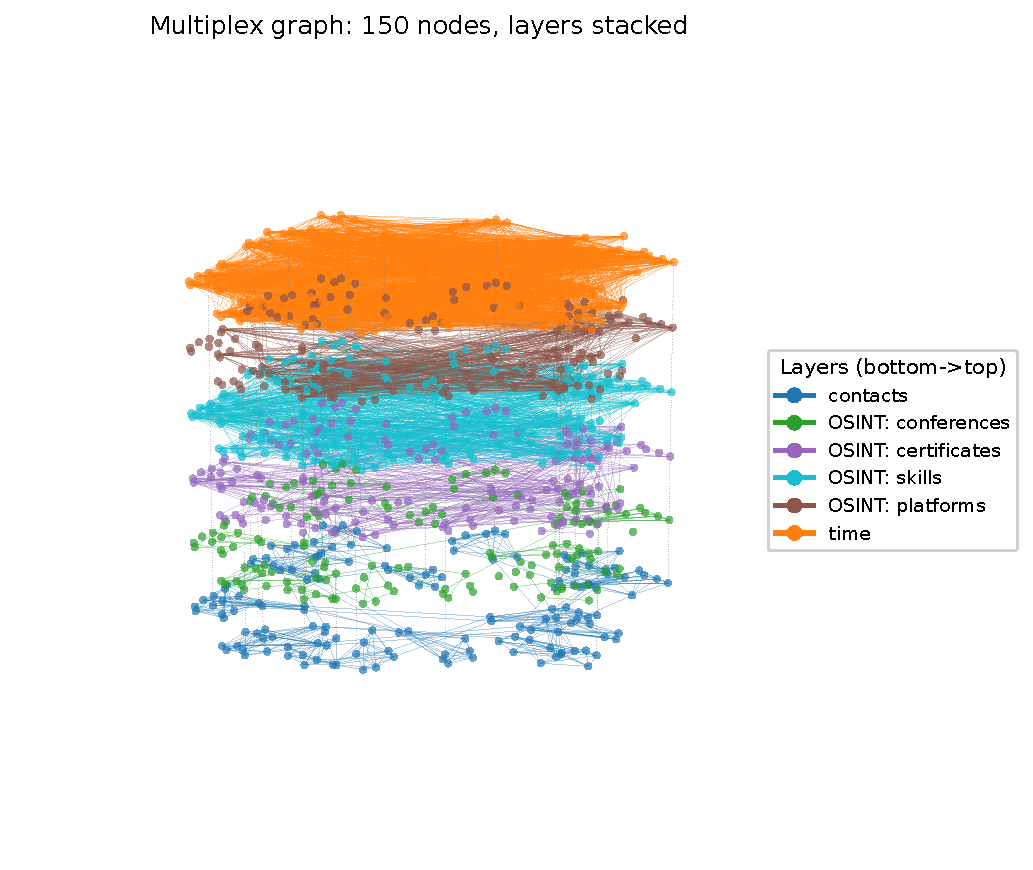
\includegraphics[width=0.72\linewidth]{fig_multiplex_3d.pdf}
\caption[Real training graph: multiplex layers]{Domain knowledge graph ($150$~nodes):
contacts, representative OSINT layers (conferences, certificates, skills, platforms), and time ---
over the \emph{same} set of accounts. Each layer carries \emph{different} connectivity, which makes
cross-layer inconsistency informative.}
\label{fig:realgraph}
\end{figure}

\subsection{Operationalizing Invariant~II: cascade and temporal GNN}
\label{sec:m-cascade}
The second invariant operates on the contacts graph $G=(V,E)$ with time divided into $T{=}28$ buckets.
An \emph{attack} is a cascade: a ``patient-zero''~$s_0$ sends malicious mail to contacts;
each recipient with probability $p_\mathrm{inf}{=}0.6$ becomes a \emph{carrier} and propagates
further to depth $H{=}4$. A single event $u\!\to\!v$ is \emph{locally} indistinguishable
from legitimate mail ($u$ \emph{is} a contact of $v$); the signal lies in the \emph{cascade context}: within the wave's window
many of $v$'s neighbors receive mail, and $u$ was hit just before
(Fig.~\ref{fig:cascade}).

\begin{figure}[t]\centering
\resizebox{0.92\columnwidth}{!}{%
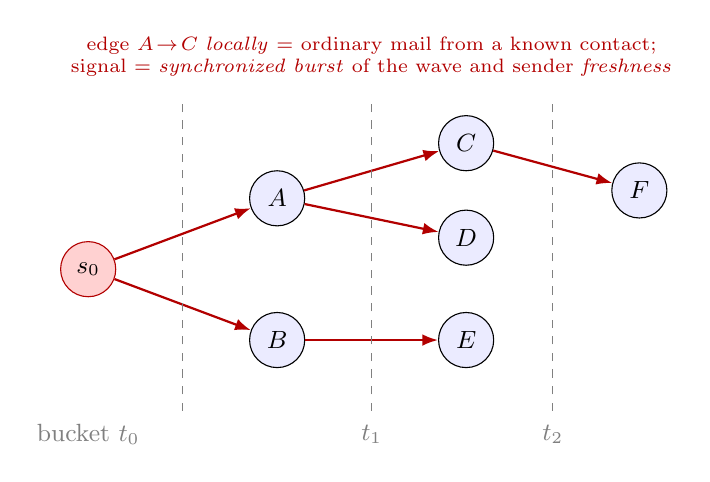
\begin{tikzpicture}[>=Latex, every node/.style={font=\small},
  acc/.style={circle, draw, minimum size=7mm, inner sep=1pt},
  inf/.style={acc, fill=red!18, draw=red!70!black},
  ben/.style={acc, fill=blue!8},
  mal/.style={-{Latex[length=2mm]}, red!70!black, thick}]
  \node[inf] (p) at (0,0) {$s_0$};
  \node[ben] (a) at (2.4,0.9) {$A$};
  \node[ben] (b) at (2.4,-0.9) {$B$};
  \draw[mal] (p)--(a); \draw[mal] (p)--(b);
  \node[ben] (c) at (4.8,1.6) {$C$};
  \node[ben] (d) at (4.8,0.4) {$D$};
  \node[ben] (e) at (4.8,-0.9) {$E$};
  \draw[mal] (a)--(c); \draw[mal] (a)--(d); \draw[mal] (b)--(e);
  \node[ben] (f) at (7.0,1.0) {$F$};
  \draw[mal] (c)--(f);
  \node[gray] at (0,-2.1) {bucket $t_0$};
  \node[gray] at (3.6,-2.1) {$t_1$};
  \node[gray] at (5.9,-2.1) {$t_2$};
  \draw[gray, dashed] (1.2,-1.8) -- (1.2,2.1);
  \draw[gray, dashed] (3.6,-1.8) -- (3.6,2.1);
  \draw[gray, dashed] (5.9,-1.8) -- (5.9,2.1);
  \node[red!70!black, align=center, font=\scriptsize] at (3.6,2.7)
    {edge $A\!\to\!C$ \emph{locally} = ordinary mail from a known contact;\\
     signal = \emph{synchronized burst} of the wave and sender \emph{freshness}};
\end{tikzpicture}}
\caption[Lateral phishing as a temporal cascade]{Lateral phishing as a temporal cascade: a carrier ($s_0$)
infects contacts, those --- their own, and the wave propagates across the graph. Detection requires \emph{multi-hop,
temporal} propagation context.}
\label{fig:cascade}
\end{figure}

\paragraph{Detectors.} We compare: \textbf{1-hop} (\texttt{LightGBM} on local features --- lower bound);
\textbf{hand-crafted cascade context} (1-hop $+$ burst/freshness/wave density ---
a strong baseline encoding the multi-hop signal by hand); \textbf{static GNN} (mean aggregation
over the contacts graph --- it sees the topology, not time); \textbf{temporal GNN (TGN-lite)}
with node memory updated bucket by bucket. Formally, the static GNN builds
embeddings from the aggregated graph with a normalized adjacency matrix $\hat{A}$ and features $X$:
\begin{equation}
H = \hat{A}\,\sigma\!\big(\hat{A}\,X\,W_1\big)\,W_2,
\qquad
\mathrm{score}_{\mathrm{stat}}(s,v) = g\!\big([\,H_s,\,H_v,\,H_s\!\odot\!H_v,\,x_{sv}\,]\big),
\label{eq:static}
\end{equation}
whereas the temporal GNN maintains a memory $m_v^{(b)}$ and scores an event of bucket~$b$ using the state
\emph{from before} its update (causality, no leakage):
\begin{align}
\mathrm{score}_{\mathrm{temp}}(s,v,b) &= g\!\big([\,m_s^{(b-1)},\,m_v^{(b-1)},\,m_s^{(b-1)}\!\odot\!m_v^{(b-1)},\,x_{sv}\,]\big),
\label{eq:temp-score}\\
m_v^{(b)} &= \mathrm{GRU}\!\Big(\tfrac{1}{d_v^{(b)}}\!\!\sum_{u:\,(u\to v)\in b}\!\!\sigma\!\big(W_m\,m_u^{(b-1)}\big),\; m_v^{(b-1)}\Big).
\label{eq:temp-mem}
\end{align}
The node features are \emph{structural} (not learning identity), which makes the model
\emph{inductive} --- it works for accounts unseen in training. Because $\mathrm{score}_{\mathrm{stat}}$
is permutation-invariant with respect to time, whereas $\mathrm{score}_{\mathrm{temp}}$ is not, the drop in
$\mathrm{AUC}_{\mathrm{temp}}$ after time shuffling \emph{measures exactly} the amount of temporal
information used --- this is the formal justification of the shuffle control.

\paragraph{Baselines for compromises.} Beyond the GNN we implement two strong, practical methods:
a \emph{volumetric baseline} in the spirit of COMPA \citep{egele2013compa,stringhini2015thataint} (a sudden spike in a
sender's sending volume within a window $W{=}2$; \texttt{IsolationForest}) and a \emph{path-based baseline} in the spirit of Hopper
\citep{ho2021hopper} (causal precursor $+$ momentum $+$ rare target). \emph{Attribution caveat:}
we implement their structural-temporal core, not the full systems --- hence we write ``volumetric''
and ``path-based''. The hyperparameters of all detectors are \emph{fixed uniformly, without
intensive tuning} (Tab.~\ref{tab:hparams}) --- no detector enjoys a tuning advantage,
which we note as a fidelity limitation and at the same time a guarantee of fairness of the comparison.

\begin{table}[t]\centering\small
\begin{tabular}{ll}
\toprule
Model / component & Hyperparameters (fixed, without tuning) \\
\midrule
GNN (static / TGN-lite / TGAT-lite) & $\mathrm{DIM}{=}24$; TGAT: $t_{\dim}{=}8$; $100$~epochs; \\
                                       & Adam $\mathrm{lr}{=}0.01$, $\mathrm{wd}{=}5\!\cdot\!10^{-4}$; dropout $0.2$ \\
GNN classifier head           & MLP, $48$ hidden units \\
Tabular detectors (LightGBM)      & $\mathrm{n\_estimators}{=}200$--$250$, $\mathrm{seed}{=}42$, \\
                                       & $\mathrm{num\_leaves}{=}31$, $\mathrm{lr}{=}0.1$ \\
volumetric (per account)                  & window $W{=}2$~buckets; IsolationForest ($150$, auto) \\
\bottomrule
\end{tabular}
\caption{Detector hyperparameters --- fixed \emph{uniformly} for all models of a given family,
framework defaults or lightly chosen, without grid search.}
\label{tab:hparams}
\end{table}

\subsection{Event model, features, and split}
\label{sec:m-events}
An event is a pair (sender~$s$, victim~$v$) with a bucket~$b$, labeled legitimate/attack, with two-sided
noise (to avoid perfect separability). \textbf{Legitimate~(0):} \emph{known} (a contact, in rhythm);
\emph{new-OSINT} (outside contacts, yet on the OSINT layer); \emph{cold} (outside all layers ---
an irreducible source of FP). \textbf{Attacks~(1):} \emph{BEC from outside the graph} (outside everything, outside the rhythm);
\emph{compromised account} (a known contact outside the rhythm). For Invariant~I we compare three feature sets
(\emph{contacts-only}, \emph{static multiplex}, \emph{full} $+$ temporal consistency)
with a \texttt{LightGBM} classifier; the split is \emph{victim-wise} (disjoint victim sets),
$20$~seeds, $95\%$ bootstrap CI for sensitivity@FPR$1\%$. For Invariant~II we use two split
regimes: \emph{victim-wise} and \emph{organization-wise} (test companies disjoint from training ones
--- \emph{inductive} validation). Headline claims are hardened over~$\ge\!20$~seeds; validations on
real graphs are reported at $8$/$5$/$3$~seeds (lower variance on a fixed structure)
with a Wilcoxon test where significance is crucial.

\subsection{Metrics, causal controls, and threats to validity}
\label{sec:m-metrics}
The headline metric is \textbf{sensitivity at FPR$=1\%$} (the operational working point):
$\text{sensitivity}@\mathrm{FPR{=}1\%} = \max\{\mathrm{TPR}(\tau):\mathrm{FPR}(\tau)\le0.01\}$;
we report AUC auxiliarily. \textbf{Note on the threshold:} real systems operate at a much stricter
FPR ($<\!4$~FP/million, \citep{ho2019detecting}), so FPR$1\%$ is a \emph{liberal lower bound}, not a deployment
threshold; at a realistic prevalence of $1{:}10^4$--$10^6$ precision follows directly from Bayes' theorem
(\ref{sec:res-rigor}). \textbf{Causal controls:} \emph{layer/rhythm shuffling} (for Invariant~I)
and \emph{temporal-order shuffling} (for Invariant~II) --- if the signal is
structural-temporal, the control must destroy the advantage (AUC$\to$random).

\paragraph{Threats to validity.} \emph{Internal}: layer redundancy (we measure Jaccard
before the gain claim) and label leakage (we separate features from the hidden infection state; the shuffle
control isolates the mechanism). \emph{External}: the population is synthetic; we validate the mechanism
on real Enron and two SNAP graphs --- the synthetic data lets us \emph{control} coverage and fabrication
at the cost of absolute effects. \emph{Construct}: sensitivity@FPR$1\%$ reflects the
low-FPR regime instead of headline AUC, in line with the caution of \citep{arp2022dos,pendlebury2019tesseract}.

% ============================================================
% Results — full synthesis of P1 (Invariant I) + P2 (Invariant II)
%          + susceptibility measurement + real-graph validation + rigor (target: C&S)
% ============================================================
\section{Results}
\label{sec:results}

We organize the results around three claims and their rigor. \emph{Invariant~I}
(\ref{sec:res-inv1}) --- cross-layer inconsistency --- detects a new sender/impersonation.
\emph{Invariant~II} (\ref{sec:res-inv2}) --- cascade dynamics --- detects a compromised account that is consistent
across all static layers and \emph{does not break down} against a stealthy attacker.
\emph{Susceptibility measurement} (\ref{sec:susceptibility}) uses these detectors as an instrument.
\emph{Real-graph validation} (\ref{sec:res-realgraphs}) and \emph{fusion with content} (\ref{sec:res-content})
test transfer and limits, while \emph{rigor} (\ref{sec:res-rigor}) determines what these numbers mean.
We report every result as AUC and sensitivity@FPR$1\%$, on a victim/organization split,
$\ge\!20$~seeds, with a causal shuffle control.

% ============================================================
\subsection{Invariant~I: cross-layer inconsistency}
\label{sec:res-inv1}
\paragraph{Multiplex vs single graph.} We compare the \emph{contacts-only} detector with the \emph{static
multiplex} (contacts $+$ eight OSINT layers from real fields). Tab.~\ref{tab:inv1}: the multiplex beats the
single graph (AUC $0.87$ vs $0.70$), and the shuffle control drops to random ($0.51$) --- the advantage
comes from real cross-layer structure, not from feature capacity. The decisive factor is the distribution
of false alarms: the contact detector flags \textbf{$100\%$} of legitimate new senders as an attack,
the multiplex --- \textbf{$0\%$} (OSINT coverage rescues a legitimate sender who shares with the victim
an observable fact). The claim is \emph{conditional}: we distinguish a legitimate new sender from an attack
when the sender shares with the victim a real domain-knowledge edge; a ``cold'' sender remains
irreducibly confusing (\ref{sec:susceptibility}). At $50\%$ OSINT edge fabrication the advantage
degrades ($0.87\!\to\!0.74$) toward the control --- false traces erode the signal.

\begin{table}[t]\centering
\begin{tabular}{lcc}
\toprule
Model & AUC & new-sender FP \\
\midrule
Contacts only & $0.70 \pm 0.01$ & $1.00$ \\
Static multiplex & $\mathbf{0.87} \pm 0.01$ & $\mathbf{0.00}$ \\
Multiplex (shuffled) & $0.51 \pm 0.01$ & --- \\
\bottomrule
\end{tabular}
\caption{Invariant~I --- multiplex vs contacts graph ($20$~seeds). Layer fusion beats the single graph
and eliminates new-sender false alarms; the advantage vanishes after shuffling.}
\label{tab:inv1}
\end{table}

\paragraph{The signal is consistency, not feature capacity.} To show this directly, we define
\emph{four explicit consistency measures} (OSINT coverage; known sender off-rhythm; new sender on OSINT;
entirely off-graph) and compare them with raw feature concatenation (Tab.~\ref{tab:consistency}).
Under logistic regression the explicit operator \emph{improves} AUC ($0.840\!\to\!0.860$), because the
linear model cannot learn the conjunction on its own; under trees the difference vanishes ($0.858$ vs $0.860$).
The four explicit measures almost match the full concatenation --- the signal is \emph{concise
consistency}, and its value is \emph{explainability and deployability}
(a single query), not higher Recall.

\begin{table}[t]\centering
\begin{tabular}{lcc}
\toprule
Model & AUC & sensitivity@FPR$1\%$ \\
\midrule
Linear $+$ concatenation & $0.840$ & $\mathbf{0.049}$ \\
Linear $+$ \textbf{consistency operator} & $\mathbf{0.860}$ & $0.019$ \\
Tree-based $+$ concatenation & $0.858$ & $\mathbf{0.066}$ \\
Tree-based $+$ consistency operator & $0.860$ & $0.034$ \\
\bottomrule
\end{tabular}
\caption{Explicit consistency operator (4~features) vs per-layer concatenation ($20$~seeds). The operator helps
the linear model and almost matches concatenation --- the signal is consistency, not capacity.}
\label{tab:consistency}
\end{table}

\paragraph{Layer ablation and selection.} Cumulative ablation (Fig.~\ref{fig:ablation}) shows that each
OSINT layer adds a little (contacts $0.57\!\to$ static $0.65$), but \emph{the temporal consistency
layer dominates}: the full model $0.86$, and removing it sets AUC back to $0.65$. Forward selection
and leave-one-out on the full set of $12$~layers (Fig.~\ref{fig:layersel}) confirm: temporal
consistency \emph{alone} reaches $0.826$ out of $0.862$ for the full model (leave-one-out $0.21$ ---
by far the most important), subsequent OSINT layers add $\sim\!0.005$ each, and the
hierarchy/domain/co-activity layers have leave-one-out $\le0.002$ (redundancy).
The \emph{minimal sufficient set} is temporal consistency $+$ $3$--$4$ OSINT layers.

\begin{figure}[t]\centering
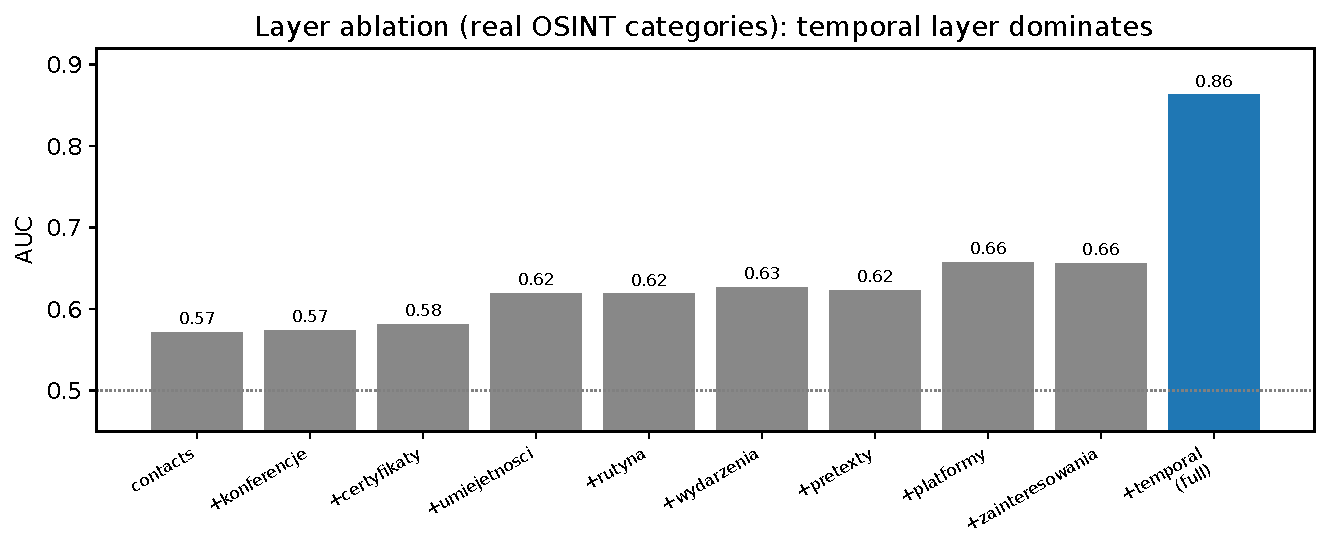
\includegraphics[width=0.8\linewidth]{fig_ablation.pdf}
\caption[Cumulative layer ablation]{Cumulative ablation. The temporal consistency layer contributes the largest
AUC gain.}
\label{fig:ablation}
\end{figure}
\begin{figure}[t]\centering
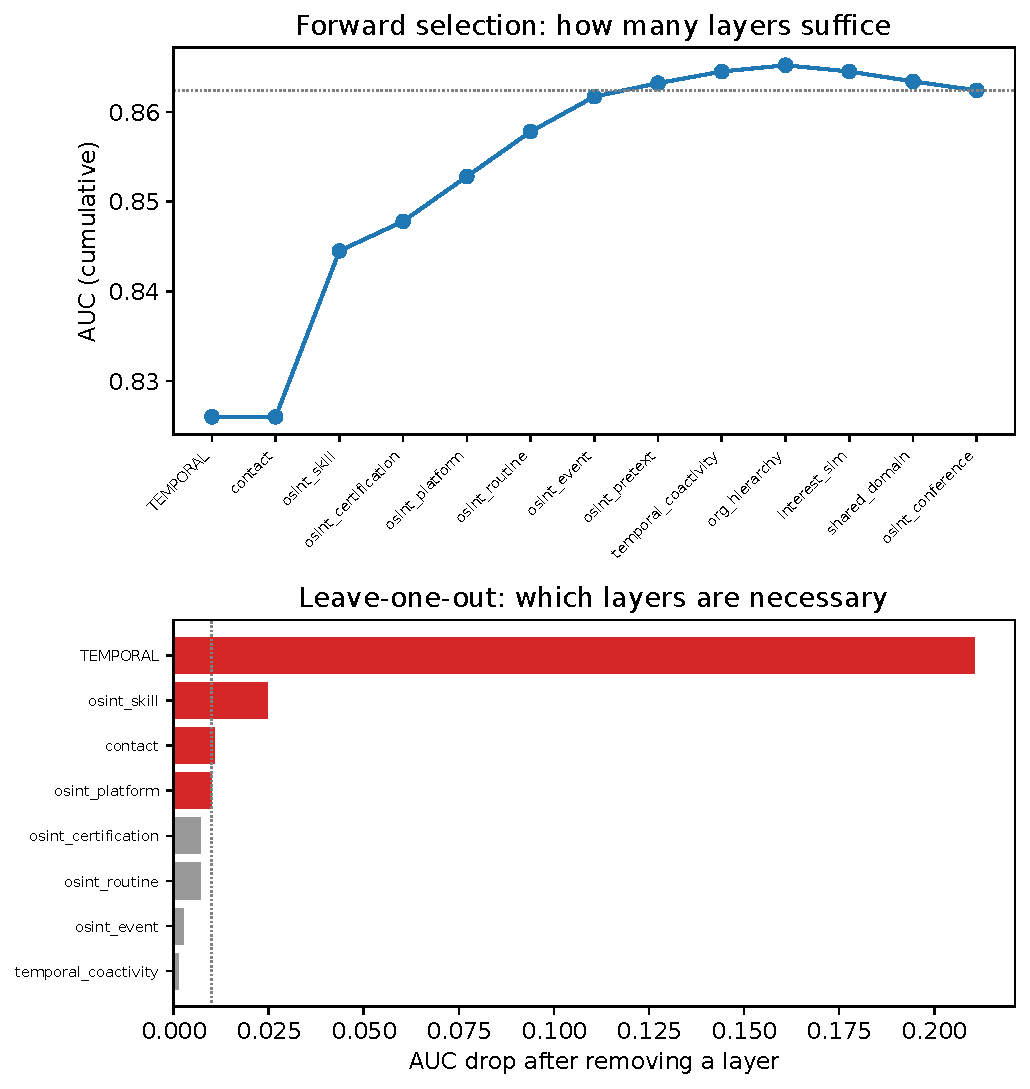
\includegraphics[width=0.9\linewidth]{fig_layer_selection.pdf}
\caption[Layer selection]{Layer selection (full set of 12). \emph{Top}: forward --- temporal
consistency alone yields most of the AUC. \emph{Bottom}: leave-one-out --- only temporal consistency (and a few
OSINT layers) is indispensable.}
\label{fig:layersel}
\end{figure}

\paragraph{Layer redundancy is a topology artifact, not a property of the method.} The high correlation of structural layers
(contacts$\approx$hierarchy$\approx$domain, Jaccard $\ge0.9$) stems from the generator (one domain per company).
By introducing a \emph{topology decorrelation} knob $\rho$ (rewiring contacts from intra-
to inter-company), we show (Tab.~\ref{tab:topo}) that already at moderate decorrelation
\textbf{Jaccard drops to $0.39$, and the independent contribution of structural layers rises to $0.25$ AUC} ---
``effectively 3--4 layers'' is a property of \emph{our} compact population, not of the multiplex as a method.

\begin{table}[t]\centering
\begin{tabular}{lccc}
\toprule
Decorrelation $\rho$ & Jaccard & indep.\ contrib.\ of structural layers & contact AUC \\
\midrule
$0.0$ (dense) & $0.93$ & $0.02$ & $0.98$ \\
$0.2$ & $0.74$ & $0.22$ & $0.78$ \\
$0.4$ & $0.59$ & $0.25$ & $0.75$ \\
$0.8$ (decorrel.) & $\mathbf{0.39}$ & $\mathbf{0.25}$ & $0.75$ \\
\bottomrule
\end{tabular}
\caption{Topology decorrelation ($20$~seeds). As layer correlation drops, the independent
contribution of the hierarchy/domain layers rises --- redundancy is an artifact of the dense corporate topology.}
\label{tab:topo}
\end{table}

\paragraph{Layers are complementary by threat.} Time dominance in the aggregate \emph{masks}
the structure: by separating the task (Fig.~\ref{fig:bythreat}), we see pure complementarity ---
for \textbf{new senders} the signal is carried by OSINT (alone $0.77$), time is useless ($0.50$);
for \textbf{compromises} the reverse holds (time $0.87$, OSINT $0.50$). Each group is indispensable for
its own failure mode. The sensitivity analysis (Fig.~\ref{fig:sensitivity}) confirms that the
\emph{ranking} (full $>$ contacts $>$ static) is qualitatively stable across the whole noise range
and for every $N\in\{40,\dots,150\}$, although the \emph{absolute} sensitivities@FPR$1\%$ are
a function of the fraction of off-rhythm mail (hence the necessary calibration on the real Enron).

\begin{figure}[t]\centering
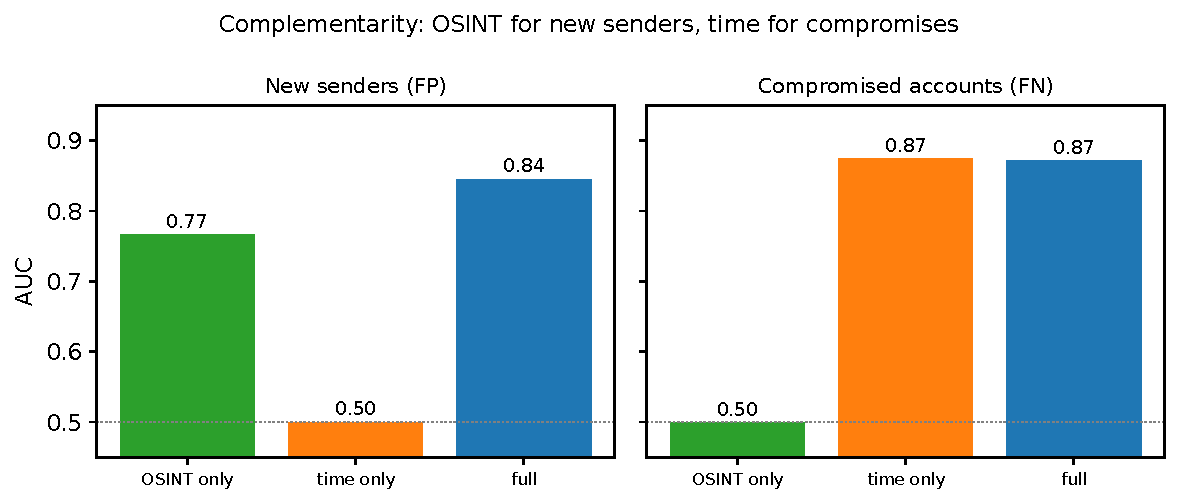
\includegraphics[width=0.8\linewidth]{fig_layer_by_threat.pdf}
\caption[Ablation per threat]{Group ablation per threat. \emph{Left}: new senders --- OSINT
indispensable, time superfluous. \emph{Right}: compromises --- the reverse. Layers are complementary.}
\label{fig:bythreat}
\end{figure}
\begin{figure}[t]\centering
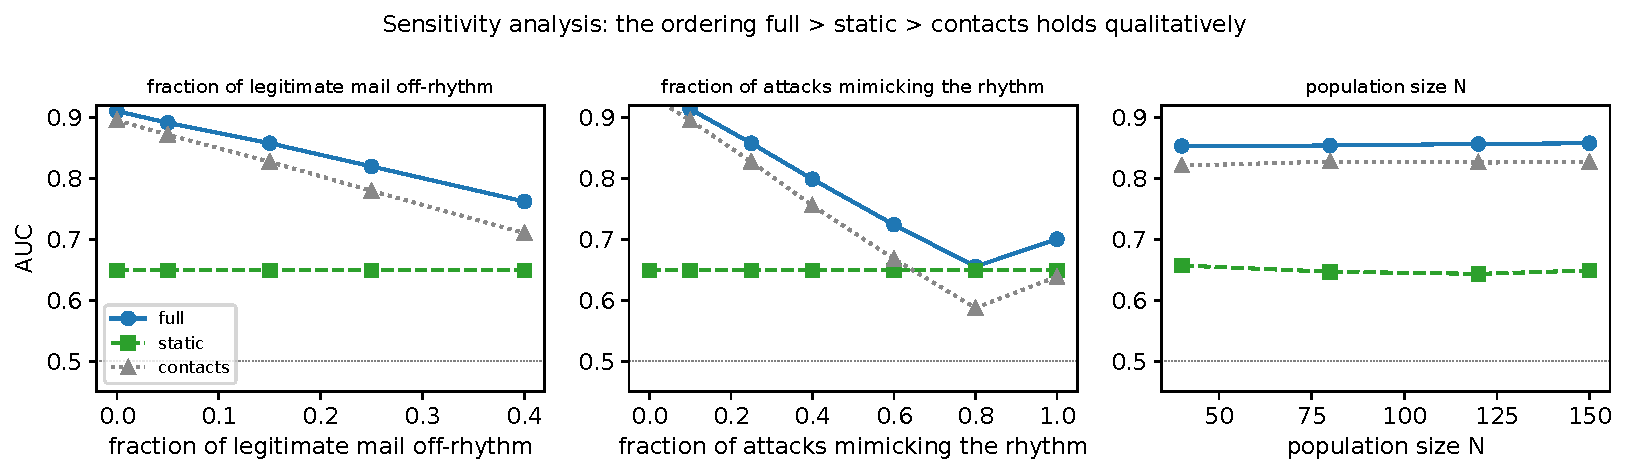
\includegraphics[width=\linewidth]{fig_sensitivity.pdf}
\caption[Sensitivity analysis]{Sensitivity (AUC). The ranking and the multiplex advantage hold
qualitatively at every noise rate and every $N$.}
\label{fig:sensitivity}
\end{figure}

\noindent\textbf{Invariant~I --- verdict.} Multiplex fusion of domain-knowledge layers beats the single graph
and eliminates new-sender false alarms; the advantage is causal (vanishes after shuffling)
and complementary to Invariant~II.

% ============================================================
\subsection{Invariant~II: temporal cascade dynamics}
\label{sec:res-inv2}
\paragraph{Detector hierarchy.} A compromised account passes \emph{all} static layers
(the multiplex is blind, AUC $0.49$); the signal lies in the dynamics. Tab.~\ref{tab:detectors} and Fig.~\ref{fig:detectors}:
1-hop features are blind ($0.70$, sensitivity@FPR$1\%\!\approx\!0$), hand-crafted multi-hop context
raises it to $0.87$, the static GNN ($0.77$) sees the topology but not time, and the \textbf{temporal
GNN} dominates: AUC $\mathbf{0.90}$, sensitivity@FPR$1\%$ $\mathbf{0.139}$. The advantage is \emph{causally
temporal}: after a time permutation the temporal GNN drops to the static level ($0.90\!\to\!0.72$, sensitivity
$0.139\!\to\!0.027$). Robustness to architecture: TGN-lite and TGAT-lite beat the hand-crafted
context in each of the $5$~seeds; the library TGN \citep{rossi2020temporal} matches it on the
operational metric --- the advantage is a property of the \emph{paradigm}, not of a specific model.

\begin{table}[t]\centering
\begin{tabular}{lcc}
\toprule
Detector & AUC & sensitivity@FPR$1\%$ \\
\midrule
1-hop (tabular)        & $0.70$ & $0.006$ \\
Static GNN               & $0.77$ & $0.063$ \\
Hand-crafted context (tab.) & $0.87$ & $0.031$ \\
\textbf{Temporal GNN}     & $\mathbf{0.90}$ & $\mathbf{0.139}$ \\
Temporal (time shuffled) & $0.72$ & $0.027$ \\
\bottomrule
\end{tabular}
\caption{Cascade detectors (victim split, $5$~seeds). Hierarchy: blind 1-hop $\to$ topology without
time $\to$ hand-crafted window $\to$ learned dynamics. Last row: time-shuffle control.}
\label{tab:detectors}
\end{table}
\begin{figure}[t]\centering
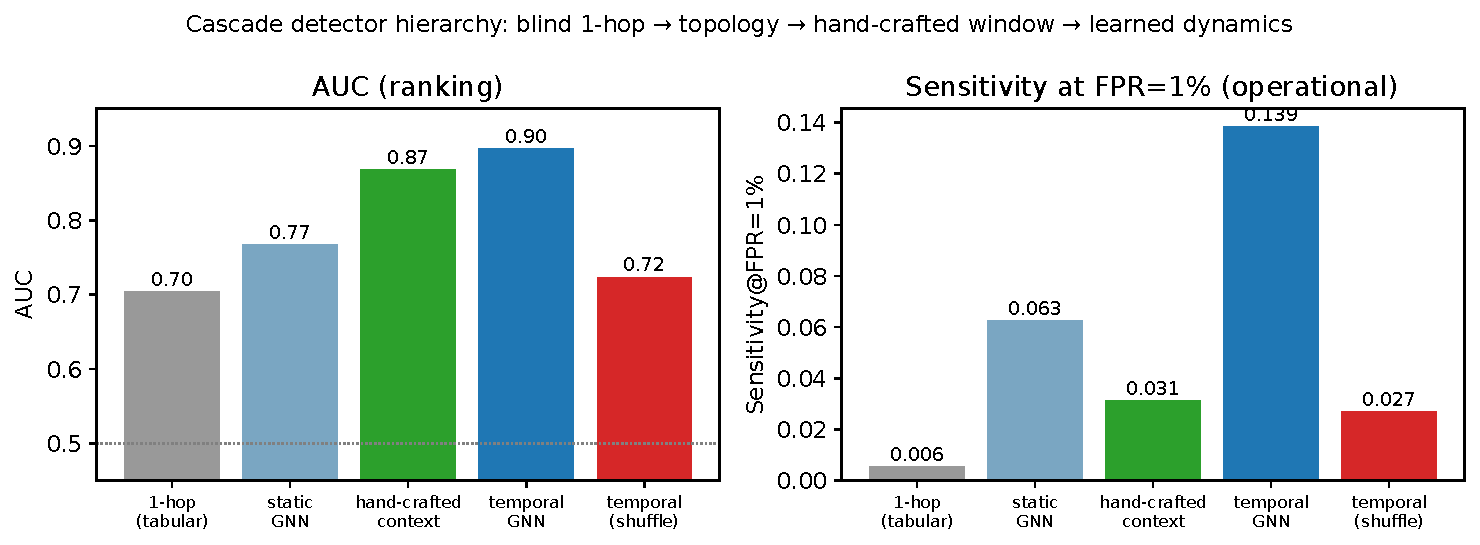
\includegraphics[width=\linewidth]{fig_cascade_detectors.pdf}
\caption[Cascade detector hierarchy]{Detector hierarchy on AUC (left) and sensitivity@FPR1\%
(right). The temporal GNN dominates; time shuffling (red) levels it with the static GNN.}
\label{fig:detectors}
\end{figure}

\paragraph{The stealthy attacker breaks volume, but not dynamics.} Against an attacker who
evades detection by spreading out sends ($K$~carriers, one per interval), the volume detector
\emph{breaks down} (AUC $0.72\!\to\!0.44$ at $K{=}1$, below random), because the sending
burst disappears; the temporal GNN \textbf{holds} (AUC $0.60$, sensitivity@FPR$1\%$ $0.039$ vs $0.017$), because it reads
the \emph{receiving side} of the cascade (Tab.~\ref{tab:stealth}, Fig.~\ref{fig:stealth}). Against the path-based
baseline (Hopper, Tab.~\ref{tab:hopper}) the path-based detector wins under extreme stealth, but degrades
with reach; \textbf{the temporal GNN is the only detector without a breakdown regime} ($0.65$--$0.82$).
The \emph{blind spot} (Tab.~\ref{tab:blindspot}): a surgical attack on \emph{a single} recipient
($p_\mathrm{inf}{=}0$, fan-out~$1$) is invisible to \emph{all} detectors (AUC $\sim\!0.46$);
the signal requires fan-out~$\ge2$ --- a precisely measured boundary of the threat model.

\begin{table}[t]\centering
\begin{tabular}{lcccc}
\toprule
& \multicolumn{2}{c}{AUC} & \multicolumn{2}{c}{sensitivity@FPR$1\%$} \\
\cmidrule(lr){2-3}\cmidrule(lr){4-5}
Level & vol. & temp. & vol. & temp. \\
\midrule
$K{=}1$ (extremely stealthy) & $0.44$ & $\mathbf{0.60}$ & $0.017$ & $\mathbf{0.039}$ \\
$K{=}2$ & $0.56$ & $\mathbf{0.75}$ & $0.021$ & $\mathbf{0.098}$ \\
$K{=}3$ & $0.58$ & $\mathbf{0.77}$ & $0.025$ & $\mathbf{0.043}$ \\
$K{=}5$ & $0.68$ & $\mathbf{0.78}$ & $0.044$ & $\mathbf{0.061}$ \\
blast  & $0.72$ & $\mathbf{0.85}$ & $0.047$ & $\mathbf{0.114}$ \\
\bottomrule
\end{tabular}
\caption{Stealthy attacker (fan-out $K$, spread over time). The volume detector breaks down
with stealth; the temporal GNN beats it at every $K\ge2$.}
\label{tab:stealth}
\end{table}
\begin{figure}[t]\centering
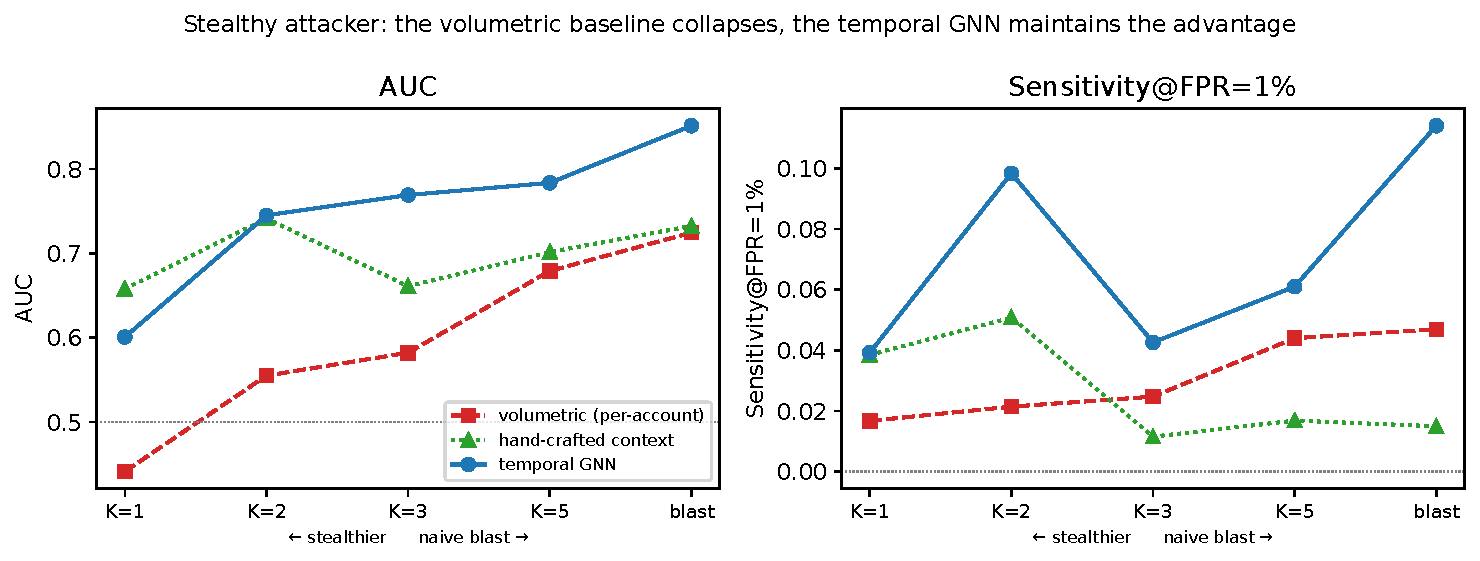
\includegraphics[width=\linewidth]{fig_cascade_stealth.pdf}
\caption[Stealth vs volume breakdown]{The stealthier the attack (smaller $K$), the more strongly the
volume detector breaks down; the temporal GNN keeps its advantage thanks to the cascade's receiving-side signal.}
\label{fig:stealth}
\end{figure}

\begin{table}[t]\centering
\begin{tabular}{lcccc}
\toprule
Level & vol. & path & manual & temp. \\
\midrule
$K{=}1$ (11\%)  & 0.48 & 0.68 & \textbf{0.76} & 0.65 \\
$K{=}2$ (27\%)  & 0.67 & 0.66 & 0.65 & \textbf{0.76} \\
$K{=}3$ (45\%)  & 0.72 & 0.61 & 0.61 & \textbf{0.78} \\
$K{=}5$ (63\%)  & 0.78 & 0.58 & 0.65 & \textbf{0.80} \\
blast (77\%)    & \textbf{0.82} & 0.59 & 0.71 & \textbf{0.82} \\
\bottomrule
\end{tabular}
\caption{Comparison with the path-based baseline (Hopper \citep{ho2021hopper}; AUC, stealth sweep~$K$).
The path-based detector wins under extreme stealth, but falls with reach; the temporal GNN holds everywhere.}
\label{tab:hopper}
\end{table}
\begin{table}[t]\centering
\begin{tabular}{lcccc}
\toprule
Fan-out & vol. & path & manual & temp. \\
\midrule
$1$ (single recipient) & 0.48 & 0.47 & 0.45 & 0.45 \\
$2$ & 0.84 & 0.51 & 0.47 & 0.77 \\
$3$ & 0.94 & 0.50 & 0.45 & 0.91 \\
$5$ & \textbf{0.98} & 0.50 & 0.50 & \textbf{0.96} \\
\bottomrule
\end{tabular}
\caption{Blind spot: attack without propagation ($p_\mathrm{inf}{=}0$), AUC vs~fan-out. With a single recipient
all detectors are random; the signal requires fan-out~$\ge2$.}
\label{tab:blindspot}
\end{table}

\paragraph{Stability and inductive generalization.} The cascade model sweep (Tab.~\ref{tab:pinf}) shows
that the hierarchy holds across the whole range $p_\mathrm{inf}\!\in\![0.05,0.9]$ and depth ---
the receiving-side signal does not vanish at a realistically low $p_\mathrm{inf}$ (temporal GNN $0.91$--$0.96$).
Inductive validation across disjoint organizations (Tab.~\ref{tab:scale}, Fig.~\ref{fig:scale}):
the operational advantage holds on \emph{unseen} companies ($4.4\times$ at $19$~companies,
$1.4\times$ at $200$), although it \emph{melts away with scale} --- the temporal GNN is a better
\emph{operational detector}, not a better \emph{ranker}.

\begin{table}[t]\centering\small
\begin{tabular}{l ccccccc}
\toprule
$p_\mathrm{inf}$ & $0.05$ & $0.1$ & $0.2$ & $0.3$ & $0.5$ & $0.7$ & $0.9$ \\
\midrule
1-hop        & $0.60$ & $0.56$ & $0.59$ & $0.60$ & $0.68$ & $0.73$ & $0.79$ \\
manual & $0.89$ & $0.87$ & $0.85$ & $0.84$ & $0.85$ & $0.87$ & $0.89$ \\
temporal   & $\mathbf{0.96}$ & $\mathbf{0.96}$ & $\mathbf{0.91}$ & $\mathbf{0.88}$ & $\mathbf{0.88}$ & $\mathbf{0.90}$ & $\mathbf{0.93}$ \\
\bottomrule
\end{tabular}
\caption{Cascade model sweep (AUC, $8$~seeds, depth~$4$). The hierarchy and the receiving-side
signal hold --- the signal is not an artifact of aggressive reach.}
\label{tab:pinf}
\end{table}
\begin{table}[t]\centering
\begin{tabular}{lcccc}
\toprule
& \multicolumn{2}{c}{AUC} & \multicolumn{2}{c}{sensitivity@FPR$1\%$} \\
\cmidrule(lr){2-3}\cmidrule(lr){4-5}
Organizations & temp. & manual & temp. & manual \\
\midrule
$19$  & $0.83$ & $0.86$ & $\mathbf{0.123}$ & $0.028$ \\
$30$  & $0.80$ & $0.86$ & $\mathbf{0.087}$ & $0.054$ \\
$200$ & $0.84$ & $0.88$ & $\mathbf{0.107}$ & $0.077$ \\
\bottomrule
\end{tabular}
\caption{Inductive validation (organization split) under increasing scale. The operational advantage
of the temporal GNN holds inductively, but melts away.}
\label{tab:scale}
\end{table}
\begin{figure}[t]\centering
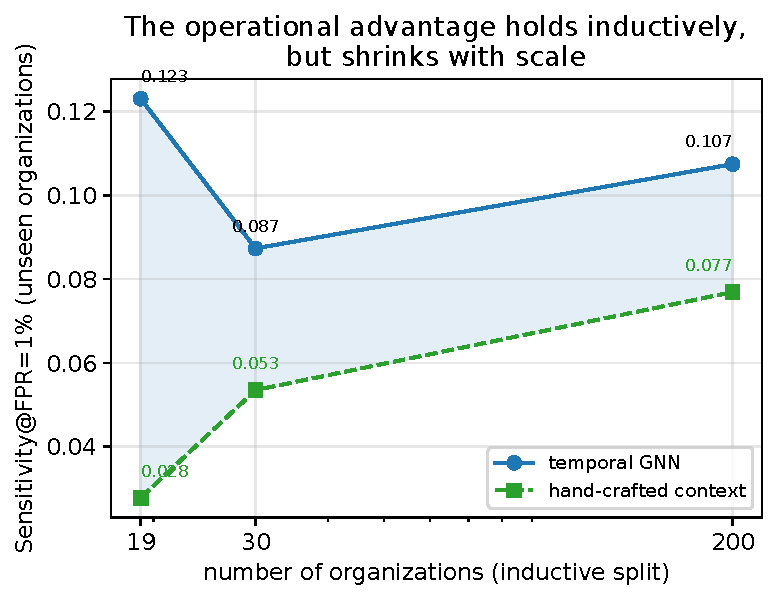
\includegraphics[width=0.62\linewidth]{fig_cascade_scale.pdf}
\caption[Inductive advantage vs scale]{sensitivity@FPR1\% on unseen organizations against the
number of companies. The advantage holds inductively, but decreases ($4.4\times\!\to\!1.4\times$).}
\label{fig:scale}
\end{figure}

\noindent\textbf{Invariant~II --- verdict.} Cascade dynamics remove the static layers' blindness to
compromises and --- unlike the volume detector --- \emph{do not break down} against a stealthy
attacker; the advantage is causally temporal and generalizes inductively.

% ============================================================
\subsection{Organization susceptibility measurement}
\label{sec:susceptibility}
The third contribution is the use of these detectors as a \emph{measuring instrument}. We define
group susceptibility as the residual margin of the fusion detector at FPR$=1\%$:
$\mathrm{Susc}(\text{group})=1-\mathrm{Recall@FPR1\%}$ (the fraction of attacks that pass; cf.\
Eq.~\ref{eq:susc}). We break down the result of the unified event model by \emph{attack channel} and victim
\emph{seniority} (Tab.~\ref{tab:susc}, $20$~seeds).

\begin{table}[t]\centering
\begin{tabular}{llcc}
\toprule
Dimension & Group & Recall@FPR$1\%$ & $\mathrm{Susc}$ \\
\midrule
\multirow{2}{*}{Attack channel}
  & External impers.\ (cold BEC) & $0.038$ & $\mathbf{0.962}$ \\
  & Compromised acct (lateral)   & $0.145$ & $0.855$ \\
\midrule
\multirow{4}{*}{\shortstack[l]{Seniority\\(lateral channel)}}
  & Executive & $\mathbf{0.076}$ & $\mathbf{0.924}$ \\
  & Senior                   & $0.135$ & $0.865$ \\
  & Mid-level & $0.162$ & $0.838$ \\
  & Junior                   & $0.160$ & $0.840$ \\
\midrule
\multirow{4}{*}{\shortstack[l]{Seniority\\(cold BEC channel)}}
  & Executive & $0.038$ & $0.962$ \\
  & Senior                   & $0.040$ & $0.960$ \\
  & Mid-level & $0.042$ & $0.958$ \\
  & Junior                   & $0.035$ & $0.965$ \\
\bottomrule
\end{tabular}
\caption{Organization susceptibility \emph{measured} by the fusion detector ($20$~seeds, FPR$=1\%$).
It is governed by the \emph{relation} (channel), not rank: cold impersonation leaves $\mathrm{Susc}\!\approx\!0.96$
regardless of level.}
\label{tab:susc}
\end{table}

\noindent Three conclusions. \emph{(1)~Susceptibility is governed by relation, not rank}: cold impersonation
leaves $\mathrm{Susc}\!\approx\!0.96$ \emph{for every} level --- no layer covers
a sender from off-graph (a structural floor of the residual $2\%$). \emph{(2)~A compromised account is less
dangerous} ($0.855$ vs $0.962$): a known contact off-rhythm is a sharp, low-FP conjunction. \emph{(3)~In the
lateral channel, rank acts \textbf{counterintuitively}}: executives, the richest in domain-knowledge layers, are
\emph{best} protected ($0.924$), while the peripheral mid/junior --- \emph{most} exposed
($0.838$/$0.840$). What protects is not status but one's own embedding in the domain-knowledge graph. The implication is
opposite to the ``VIP-first'' program: under a lateral threat, the largest margin lies on the periphery.

% ============================================================
\subsection{Validation on real communication graphs}
\label{sec:res-realgraphs}
We validate the mechanisms on \emph{real} graphs (Enron, two SNAP graphs), where the structure
and rhythms are real, and the attack labels are controlled injections (a matched design: legitimate traffic and attack
are edges with the same distribution of endpoints/degrees, distinguished solely by their temporal
pattern).

\paragraph{Invariant~I on the real Enron multiplex.} From the headers we build a real structural-temporal
multiplex (contacts, co-recipients, domain, rhythm; OSINT remains synthetic --- a deliberate
split). On $818$~senders and $\sim\!170$k~events, the full multiplex reaches AUC $0.94$
(legitimate traffic on-rhythm) versus $0.75$ for contacts alone. The \emph{off-hours traffic} audit
(Fig.~\ref{fig:enronaudit}) shows that the operational sensitivity was inflated: a realistic
figure is $\sim\!0.49$ (not $0.87$), but the multiplex \emph{advantage} over the temporal layer alone
\emph{rises} with the off-hours fraction. The sharpest control --- the \emph{temporal split} of rhythm
estimation (rhythm from the early $60\%$, evaluation on the later $40\%$) together with off-hours
traffic (Tab.~\ref{tab:enronsplit}): the temporal layer \emph{alone} collapses operationally (Recall@FPR$1\%\!\to\!0$),
but \textbf{the full multiplex remains robust} (AUC $0.84$, Recall $0.51$), and its advantage over time
\emph{rises} after the leakage is removed --- the structural signal is real.

\begin{table}[t]\centering
\begin{tabular}{lcccc}
\toprule
 & \multicolumn{2}{c}{temporal layer} & \multicolumn{2}{c}{full multiplex} \\
\cmidrule(lr){2-3}\cmidrule(lr){4-5}
Rhythm estimated from & AUC & R@FPR$1\%$ & AUC & R@FPR$1\%$ \\
\midrule
full history (\emph{with leakage}) & $0.86$ & $0.73$ & $0.94$ & $0.88$ \\
early window (\emph{temporal split}) & $0.75$ & $0.00$ & $0.87$ & $0.51$ \\
early window $+\,$off-hours (\emph{both}) & $0.68$ & $\mathbf{0.00}$ & $\mathbf{0.84}$ & $\mathbf{0.51}$ \\
\bottomrule
\end{tabular}
\caption{Rhythm leakage control on Enron ($20$~seeds). The temporal layer alone is inflated by leakage
(Recall$\to0$), but the full multiplex remains robust under \emph{both} controls.}
\label{tab:enronsplit}
\end{table}
\begin{figure}[t]\centering
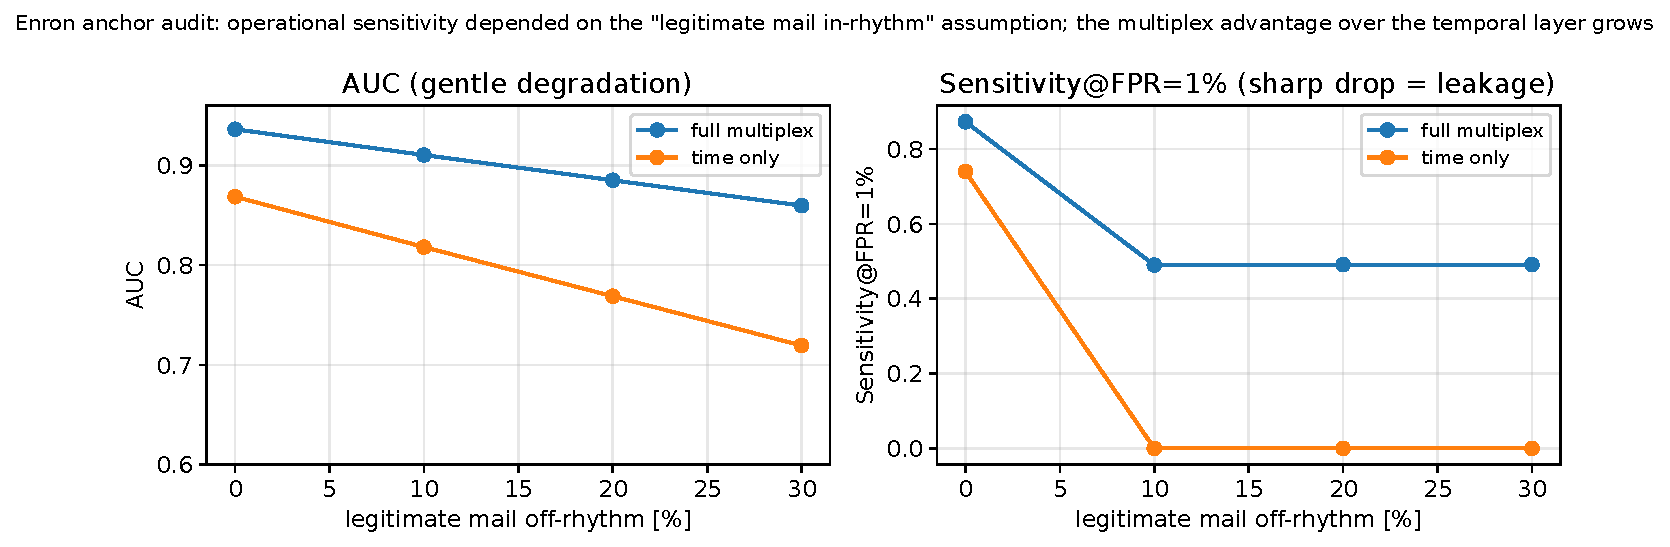
\includegraphics[width=\linewidth]{fig_enron_audit.pdf}
\caption[Enron anchor audit]{Enron anchor audit. AUC (left) degrades gently with the off-hours
traffic fraction; the operational sensitivity@FPR1\% (right) was inflated --- the temporal layer alone collapses
to zero, the multiplex advantage rises.}
\label{fig:enronaudit}
\end{figure}

\paragraph{Invariant~II on the real Enron topology.} Repeating the cascade experiment on the real graph
($1990$~accounts, $8$~seeds, leak-free), the hierarchy from the synthetic data \emph{is reproduced} (Tab.~\ref{tab:enron-casc},
Fig.~\ref{fig:enron-casc}): 1-hop $0.65$, manual $0.77$, \textbf{temporal GNN $0.85$} (beats manual
in $8/8$~seeds), and time shuffling levels it with manual ($0.77$) --- the advantage is causally
temporal on the real topology as well.

\begin{table}[t]\centering
\begin{tabular}{lcc}
\toprule
Detector & AUC & sensitivity@FPR$1\%$ \\
\midrule
1-hop (tabular)        & $0.65$ & $0.022$ \\
Hand-crafted context (tab.) & $0.77$ & $0.042$ \\
\textbf{Temporal GNN}     & $\mathbf{0.85}$ & $\mathbf{0.072}$ \\
Temporal (time shuffled) & $0.77$ & $0.049$ \\
\bottomrule
\end{tabular}
\caption{Invariant~II on the REAL Enron contacts graph ($1990$~nodes, matched design,
$8$~seeds). The temporal GNN beats the manual and shuffled variants in $8/8$~seeds.}
\label{tab:enron-casc}
\end{table}
\begin{figure}[t]\centering
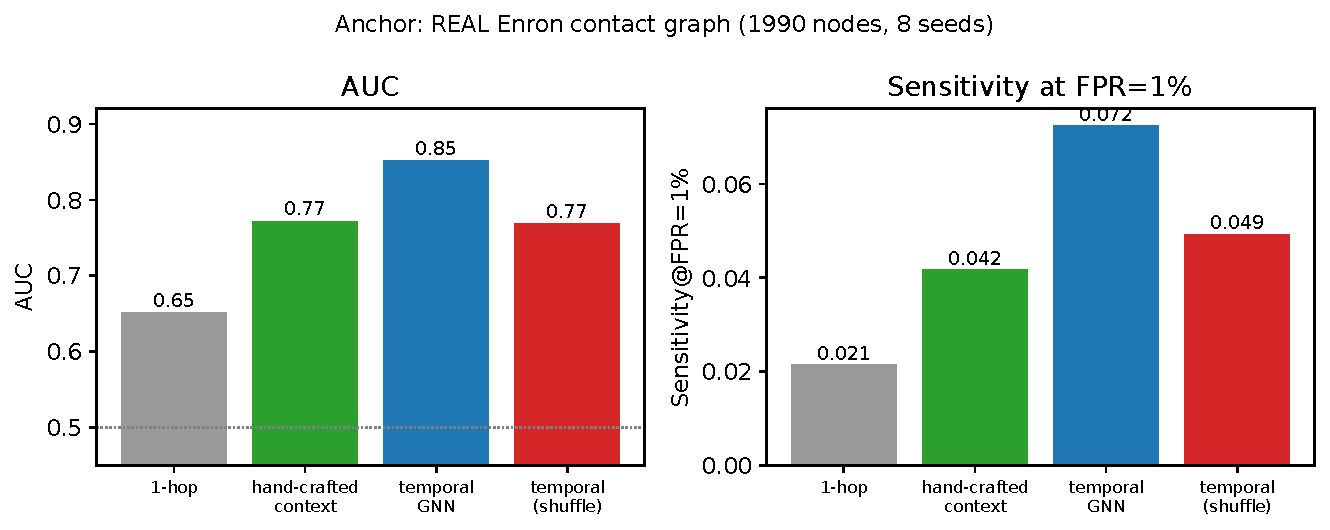
\includegraphics[width=\linewidth]{fig_cascade_enron.pdf}
\caption[Cascade anchor on Enron]{Invariant~II on Enron: the same hierarchy as on synthetic data
(1-hop $<$ manual $<$ temporal), with a shuffle control leveling the temporal
with the manual.}
\label{fig:enron-casc}
\end{figure}

\paragraph{Transfer to two further SNAP graphs.} On \texttt{email-Eu-core} \citep{paranjape2017motifs} and \texttt{CollegeMsg}
\citep{panzarasa2009patterns} (\citep{leskovec2014snap}) the regime transition \emph{replicates}
(Tab.~\ref{tab:realgraphs}, Fig.~\ref{fig:realgraphs}): against the naive blast the volume detector dominates ($0.97$),
but against a \emph{stealthy} attacker it breaks down ($0.70$/$0.66$), while the temporal GNN holds
($0.88$/$0.85$). The predictivity probe is therefore positive: the method ranking established on one topology
\emph{transfers} --- the mechanism is not an artifact of a single corpus (on the three real graphs
the Wilcoxon test of temporal vs random gives $p<0.001$).

\begin{table}[t]\centering
\begin{tabular}{llcccc}
\toprule
& & \multicolumn{2}{c}{AUC} & \multicolumn{2}{c}{sensitivity@FPR$1\%$} \\
\cmidrule(lr){3-4}\cmidrule(lr){5-6}
Graph & Regime & vol. & temp. & vol. & temp. \\
\midrule
\multirow{2}{*}{\texttt{email-Eu-core}} & blast  & $\mathbf{0.97}$ & $0.70$ & $\mathbf{0.29}$ & $0.06$ \\
                                        & stealthy   & $0.70$ & $\mathbf{0.88}$ & $0.00$ & $\mathbf{0.08}$ \\
\midrule
\multirow{2}{*}{\texttt{CollegeMsg}}    & blast  & $\mathbf{0.97}$ & $0.70$ & $\mathbf{0.35}$ & $0.04$ \\
                                        & stealthy   & $0.66$ & $\mathbf{0.85}$ & $0.02$ & $\mathbf{0.12}$ \\
\bottomrule
\end{tabular}
\caption{Transfer to two real SNAP graphs ($3$~seeds). Naive blast: the volume detector wins.
Stealthy attack: the volume detector breaks down, the temporal GNN holds --- as on Enron and the synthetic data.}
\label{tab:realgraphs}
\end{table}
\begin{figure}[t]\centering
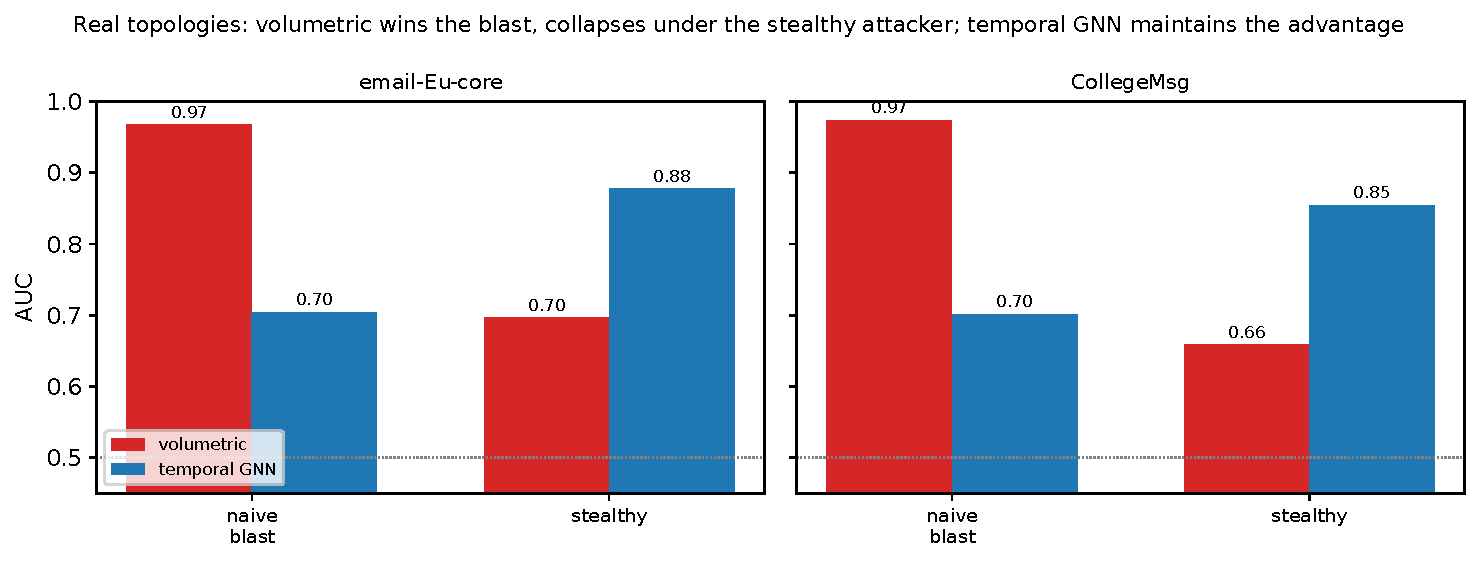
\includegraphics[width=\linewidth]{fig_cascade_realgraphs.pdf}
\caption[Replication on real topologies]{Two real topologies. The volume detector (red) wins the naive
blast, but breaks down under the stealthy attack; the temporal GNN (blue) maintains its
effectiveness.}
\label{fig:realgraphs}
\end{figure}

% ============================================================
\subsection{Fusion with content and the graph boundary}
\label{sec:res-content}
The invariants are blind to cold off-graph impersonation (\ref{sec:susceptibility}); that is the
domain of content. Combining the graph signal with content (TF-IDF) in two regimes
(Tab.~\ref{tab:content}): in the \emph{tell-tale} regime content separates almost perfectly ($0.997$),
and the multiplex is redundant; in the \emph{mimicry} regime (BEC) content is blind ($0.502$),
and the signal is carried by the multiplex ($0.862$). \emph{Fusion} yields best-of-both ($0.998$/$0.848$) --- content
and graph are complementary. \emph{GNN sanity check}: on a small graph ($N{=}150$) a single untuned
multiplex GNN does \emph{not} surpass the explicit hand-crafted features (AUC $0.78$ vs $0.86$ LightGBM) ---
at this scale the explicit membership features already capture the signal; the advantage of a learned
representation we defer to larger graphs.

\begin{table}[t]\centering
\begin{tabular}{lccc}
\toprule
Regime & Content only & Multiplex only & Fusion \\
\midrule
Tell-tale (content trace) & $\mathbf{0.997}$ & $0.862$ & $0.998$ \\
Mimicry (BEC) & $0.502$ & $0.862$ & $\mathbf{0.848}$ \\
\bottomrule
\end{tabular}
\caption{Fusion of content with the multiplex (AUC; $20$~seeds). Content wins tell-tale, the multiplex
wins mimicry, fusion combines both.}
\label{tab:content}
\end{table}

% ============================================================
\subsection{Rigor: what it means for a detector to ``work''}
\label{sec:res-rigor}
\paragraph{The whole curve and significance.} Instead of a single threshold we report the
sensitivity--FPR curve (Fig.~\ref{fig:fpr}) and a paired test. At a realistically low FPR ($0.1\%$) all methods
are weak --- we do not hide this. Hardening the main contrast on~$20$~seeds (the stealthy point,
Tab.~\ref{tab:headline-ci}): the receiving-side signal beats the volume detector \emph{significantly and with a large effect}
(temporal GNN $+0.081$ AUC, $p<0.001$, Cliff~$\delta{=}0.88$); the advantage of the learned GNN \emph{over} the hand-crafted
context is \emph{operating-point dependent} and insignificant in key regimes. The credible result
is therefore not ``the GNN beats everything'', but that \emph{under a stealthy attack the receiving-side signal} (learned
\emph{or} hand-crafted) significantly surpasses volume detection, which breaks down.

\begin{table}[t]\centering
\begin{tabular}{lccc}
\toprule
Contrast (stealthy attack) & $\Delta$AUC & paired $p$ & Cliff~$\delta$ \\
\midrule
temporal GNN $>$ volume        & $+0.081$ & $<\!0.001$ & $0.88$ (large) \\
temporal GNN $>$ hand-crafted context   & $+0.064$ & $<\!0.001$ & $0.78$ (large) \\
hand-crafted context $>$ volume            & $+0.017$ & $0.28$     & $0.28$ (small, n.s.) \\
\bottomrule
\end{tabular}
\caption{Hardening of the main contrast on~$20$~seeds (the stealthy point). Paired Wilcoxon $+$ Cliff~$\delta$.}
\label{tab:headline-ci}
\end{table}
\begin{figure}[t]\centering
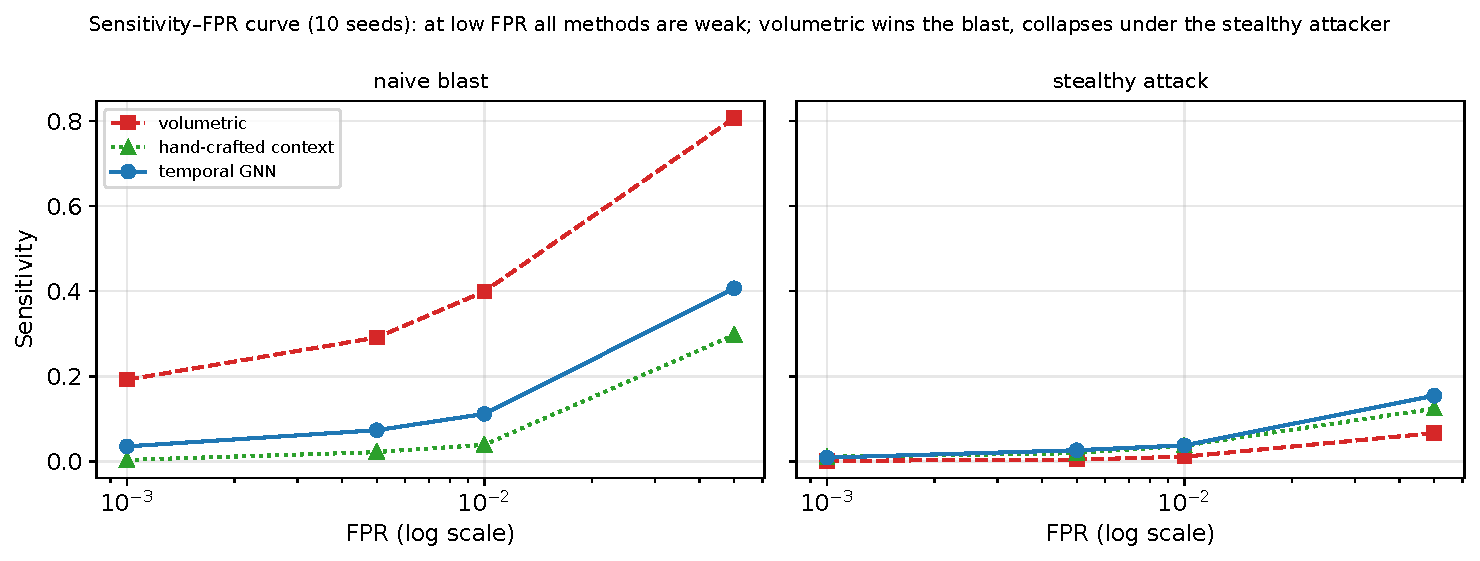
\includegraphics[width=\linewidth]{fig_cascade_fpr.pdf}
\caption[Sensitivity--FPR curve]{Sensitivity--FPR curve ($10$~seeds). At low FPR all
methods are weak; the volume detector dominates the blast and breaks down under the stealthy attack, where the
receiving-side signal holds.}
\label{fig:fpr}
\end{figure}

\paragraph{Base rate: why this is a lower bound.} Sensitivity at a given FPR is
independent of prevalence, but \emph{precision} drops when the attack is rare. From Bayes' theorem
$\mathrm{prec}(b)=rb/(rb+\alpha(1-b))$ (\ref{eq:baserate}): for the operating point sensitivity $0.14$ at
FPR$1\%$ and a real prevalence of $1{:}10^4$, each detected attack comes with $\sim\!700$ false alarms
(Tab.~\ref{tab:baserate}) --- about $\sim\!3$~orders too high relative to the threshold of \citet{ho2019detecting}
($<\!4$/million). \textbf{Consequence:} at a real prevalence our detectors --- and any
detector with a similar ROC curve --- are a \emph{triage and ranking} tool, not an autonomous
defense; we locate the contribution in the signal, the mechanism, and the methodology.
\begin{equation}
\mathrm{prec}(b) \;=\; \frac{r\,b}{r\,b + \alpha\,(1-b)}.
\label{eq:baserate}
\end{equation}

\begin{table}[t]\centering
\begin{tabular}{lccc}
\toprule
Attack frequency & Precision & FP per attack & FP/million \\
\midrule
$1{:}3$ (evaluation) & 0.82 & $\sim$0 & 7\,500 \\
$1{:}100$           & 0.12 & 7        & 9\,900 \\
$1{:}1000$          & 0.014 & 71      & 9\,990 \\
$1{:}10\,000$       & 0.001 & 714     & 9\,999 \\
$1{:}10^6$          & $<$0.001 & 71\,000 & 10\,000 \\
\bottomrule
\end{tabular}
\caption{Base-rate arithmetic for the temporal GNN operating point (sensitivity $0.14$,
FPR$1\%$). Precision follows from the ROC curve, independently of the model.}
\label{tab:baserate}
\end{table}

\paragraph{Label noise --- the price of learning.} Flipping an increasing fraction of training labels
(Tab.~\ref{tab:labelnoise}), the learned GNN degrades \emph{fastest} (temporal $0.82\!\to\!0.70$ at
$20\%$ noise, volume only $0.79\!\to\!0.75$) --- under realistic label noise the advantage of the learned
model shrinks. This is another boundary that we state explicitly.

\begin{table}[t]\centering
\begin{tabular}{lcccc}
\toprule
Label noise & vol. & path & manual & temp. \\
\midrule
$0\%$   & $0.79$ & $0.72$ & $0.66$ & $\mathbf{0.82}$ \\
$5\%$   & $0.78$ & $0.71$ & $0.65$ & $\mathbf{0.80}$ \\
$10\%$  & $0.78$ & $0.71$ & $0.64$ & $\mathbf{0.76}$ \\
$20\%$  & $\mathbf{0.75}$ & $0.68$ & $0.62$ & $0.70$ \\
\bottomrule
\end{tabular}
\caption{Audit of noisy training labels (AUC, stealthy attack). The learned GNN degrades fastest ---
sensitivity to noise is the price of learning.}
\label{tab:labelnoise}
\end{table}

\noindent\textbf{Definition of effectiveness.} A method ``works'' \emph{operationally} if its advantage is
causally relational-temporal (it vanishes under shuffle controls), transferable across topologies
(predictivity probe), and measured at low FPR with explicit prevalence arithmetic. Under this
definition ``$98\%$ on a mass benchmark'' does not attest to detecting spear phishing --- what counts is
sensitivity to the \emph{residual} $2\%$, with an explicitly stated floor (cold impersonation)
and an honest threshold.

% ============================================================
% Discussion --- interpretation, implications, limitations (target: C&S)
% ============================================================
\section{Discussion}
\label{sec:discussion}

The results converge on a single thesis: residual spear phishing is detectable
exactly to the degree to which it \emph{violates} the victim's observable domain knowledge ---
and that degree can be \emph{measured}. Below we interpret the mechanism, outline the
practical implications, and honestly delineate the limits.

\subsection{Interpretation: two invariants, two failure modes}
The two invariants are not competing detectors but \emph{complementary} responses to two
disjoint modes of targeted attack. The cross-layer inconsistency invariant
(\ref{sec:res-inv1}) addresses the \emph{new sender}: role or authority impersonation is
``known'' in one layer (e.g.\ name, domain), yet inconsistent in others (no OSINT trace, no
relationship history) --- which breaks the pattern of a genuine relationship that is consistent across many layers at once.
The cascade dynamics invariant (\ref{sec:res-inv2}) addresses the \emph{compromised account}, which is
consistent across all static layers (because it \emph{is} a genuine contact), yet betrays itself
\emph{temporally}: it sends out of rhythm, creating a recipient-side cascade. The per-threat
ablation makes this complementarity explicit: for new senders the signal is carried by
OSINT, while time is useless; for compromises it is the reverse. This observation explains
why single approaches (a content filter alone, a contact graph alone, a volumetric detector alone) fail
on the residual $2\%$: each is blind to one of the two modes.

Mechanistically, the most important result concerns the \emph{stealthy attacker}. A volumetric detector
(in the spirit of COMPA \citep{stringhini2015thataint}) assumes that a compromise manifests as a ``surge'';
when the attacker deliberately spreads out the sending, the volumetric signal vanishes (AUC below random).
Cascade dynamics reads the \emph{recipient side} --- the wave-like signature among the neighbors ---
whose stealth the sender cannot hide. This is consistent with the observations of Ho et al.\ \citep{ho2019detecting},
that lateral phishing requires a signal beyond the content of a single message; we differ, however,
in that we locate the signal in the \emph{dynamics of the domain knowledge graph}, not in headers or relays.

\subsection{Practical implications}
The strongest implication stems from the susceptibility measurement (\ref{sec:susceptibility}) and is \emph{counter-intuitive}.
Typical defense programs prioritize ``VIPs'' (executives) as the most exposed. Our
measurement shows that with respect to the \emph{lateral} channel the opposite holds: executives, densely embedded
in the domain knowledge graph, are \emph{best} protected by the structural signal alone, while the largest
unaddressed margin lies on the \emph{periphery} (mid/junior). The recommendation is therefore two-part:
(a)~awareness programs and hard controls (e.g.\ out-of-band verification for transfers) should
cover the \emph{periphery}, not just the top; (b)~detection resources are worth directing where the domain knowledge
graph is sparse --- because that is where the residual margin is largest. With respect to the
\emph{cold impersonation} channel the measurement delivers a hard message: no relational layer suffices
($\mathrm{Susc}\!\approx\!0.96$ regardless of rank), so here the graph \emph{must} be combined
with content and process controls --- as the fusion experiment confirms. This makes the domain knowledge graph
not a standalone product but a \emph{prioritization layer}: it indicates who, and through which relationship,
is most weakly protected.

The result also has an implication for the human factor. Because human susceptibility rises under
time pressure and authority cues while awareness training moderates it only partially
(Section~\ref{sec:related}), a structural susceptibility measure allows limited training interventions
to be \emph{targeted} at the roles that the technology protects most weakly.

\subsection{Limitations}
We treat the limitations seriously, because they define the scope of the claims. \emph{First,
maliciousness is synthetic.} No public corpus links real OSINT facts with labeled compromises;
we generate attack labels on real structure (Enron, SNAP) or on a synthetic population of twins.
We therefore validate the \emph{mechanism} (out-of-rhythm mail separates compromises; layer
inconsistency separates impersonation), not the detection of real intrusions. The OSINT multiplex
advantage (Invariant~I) remains \textbf{exclusively synthetic} --- we read it
as a proof of soundness, not a measurement on real traffic. We also note a degree of
\emph{circularity}: the synthetic population is generated graph-first, so detecting a violation of that
structure is in part built in. Consistent with this, the layer analysis (\ref{sec:res-inv1}) shows the
\emph{temporal} layer carries almost all of Invariant~I's signal, the structural and OSINT layers
contributing little unless the topology is artificially decorrelated; the headline of Invariant~I thus
reduces, in practice, to ``rhythm consistency detects off-rhythm mail'', whereas the cascade result
(Invariant~II) establishes the receiving-side signal far more robustly on real graphs. \emph{Second, the susceptibility measurement
inherits these assumptions}: the $\mathrm{Susc}$ figures are relative to our event model
and population structure (19~companies~$\times\sim$8~people, one domain per company); the direction of the conclusions
(relationship~$>$~rank; periphery most exposed) is qualitatively robust, but the exact values
are not directly transferable to every organization. The direction is moreover partly
\emph{definitional}: executives are layer-rich \emph{by construction}, so their stronger structural
protection follows in part from how we tied layer richness to seniority --- a coupling that should be
stress-tested under alternative assignments before the ``periphery first'' recommendation is generalized. \emph{Third, the scale is limited}
($N{=}150$ twins; real graphs up to~$\sim$2k nodes), so the comparison
with heavy GNN architectures (GATNE/HGT) is treated as a sanity check, not a full benchmark.
\emph{Fourth, the operational threshold}: even the best operating point (sensitivity@FPR$1\%$) remains
orders of magnitude away from the deployment threshold on real mail (Ho et al.\ \citep{ho2019detecting}:
$<\!4$~FP/M); we report it as a \emph{requirement we are beginning to meet}, not an absolute record.

\subsection{Future work directions}
\begin{itemize}[noitemsep,topsep=2pt]
  \item \textbf{Real BEC labels.} The most important next step is validation on a corpus
  with labeled, real compromises --- to turn the proof of mechanism into a measurement of detectability.
  \item \textbf{A learned, inductive domain knowledge graph.} Replacing the hand-crafted consistency features
  with a learned multiplex GNN with explicit cross-layer consistency regularization, validated
  inductively on unseen organizations.
  \item \textbf{Adaptive attack and drift.} Studying an attacker that \emph{learns}
  the domain knowledge graph (LLM~$+$~OSINT \citep{bethany2024evaluating}) and tunes rhythm/relationships, as well as population drift
  over time (TESSERACT \citep{pendlebury2019tesseract}).
  \item \textbf{Susceptibility as a steering signal.} Using the measured $\mathrm{Susc}$ for
  dynamic prioritization of controls and personalization of training --- with an evaluation of whether it lowers the real
  click-through rate.
\end{itemize}

% ============================================================
% Conclusions (target: Computers & Security)
% ============================================================
\section{Conclusions}
\label{sec:conclusion}

Modern phishing detection works in aggregate, yet a residual fraction, spear phishing and BEC, remains the most
costly and almost invisible to content filters. We have argued that this is a structural property: a targeted
attack succeeds by respecting the victim's domain knowledge, so the maliciousness signal lies not in the content
but in its inconsistency with the graph of that knowledge and in the dynamics of its violation.

\paragraph{Answers to the research questions.}
\begin{description}[noitemsep,topsep=2pt]
  \item[RQ1 (static signal, T1):] Yes, conditionally. The cross-layer inconsistency invariant beats a single
  contact graph and removes false alarms from legitimate new senders (Section~\ref{sec:res-inv1}), provided there
  is a shared, observable domain-knowledge edge, and the gain vanishes under the layer/rhythm shuffle control.
  \item[RQ2 (temporal signal, T2):] Yes. The temporal invariant removes the blindness of the static layers and,
  unlike a volume-based detector, does not collapse against a stealthy attacker (Section~\ref{sec:res-inv2}); the
  advantage is causally temporal and transfers to three real graphs.
  \item[RQ3 (measurement, T3):] Measurable, and governed by relation rather than rank. Cold external impersonation
  leaves a margin of $\mathrm{Susc}\!\approx\!0.96$ at every level, whereas in the lateral channel it is the
  periphery that is most exposed, not the executives (Section~\ref{sec:susceptibility}). At a realistic base rate
  the detectors act as a triage instrument, with effectiveness defined operationally through low-FPR sensitivity
  under leak controls and a predictivity probe (Section~\ref{sec:res-rigor}).
\end{description}

\paragraph{Contributions.}
\begin{enumerate}[noitemsep,topsep=2pt]
  \item The concept and formalization of the domain knowledge graph, with the thesis that spear phishing is its
  violation, uniformly for lateral/BEC and external impersonation.
  \item Two complementary detection invariants (cross-layer inconsistency and cascade dynamics), with causal
  controls and validation on three real communication graphs.
  \item A measured organizational susceptibility metric showing that the residual margin is governed by relation,
  and that in the lateral channel the periphery is more exposed than the top.
  \item A leak-aware evaluation methodology and an operational definition of spear-phishing detection
  effectiveness.
\end{enumerate}

\paragraph{Limitations (summary).} The maliciousness is synthetic, so we validate the mechanism rather than the
detection of real intrusions; the susceptibility measurement inherits the assumptions of the event model; and
scale and the operational threshold remain limitations. Section~\ref{sec:discussion} gives the details.

The contribution is a concept, a method, and a measurement discipline, rather than a finished product. Spear
phishing is a violation of domain knowledge, and the graph of that knowledge makes both the attack and the
susceptibility to it measurable. This points toward a defense that asks not whether a message looks malicious but
whether it is consistent with what the organization knows about itself.


%% ==== Back matter: required declarations (C&S Guide for Authors) ====
\section*{CRediT authorship contribution statement}
\textbf{Kamil Warpechowski:} Conceptualization, Methodology, Software, Investigation, Validation,
Writing -- original draft. \textbf{Bogdan Ksi{\k{e}}{\.z}opolski:} Supervision, Conceptualization,
Writing -- review \& editing.

\section*{Declaration of competing interests}
The authors declare that they have no known competing financial interests or personal relationships
that could have appeared to influence the work reported in this paper.

\section*{Funding}
% TODO: confirm with co-author/NASK whether a specific grant supported this work; replace if so.
This research did not receive any specific grant from funding agencies in the public, commercial,
or not-for-profit sectors.

\section*{Data availability}
% TODO before submission: replace XXXXXXX with the DOI reserved on Zenodo
% (New upload -> "Reserve DOI"); the same DOI is recorded in CITATION.cff and .zenodo.json.
The reproducibility package --- the synthetic population generator, all experiment and analysis code,
the generated population of $150$~personas, and the computed results from which the tables and figures
are produced --- is openly archived on Zenodo (DOI:~\texttt{10.5281/zenodo.XXXXXXX}). The real
communication graphs used for validation are public: the Enron email corpus \citep{klimt2004enron}
and the SNAP datasets \texttt{email-Eu-core} and \texttt{CollegeMsg} \citep{leskovec2014snap}.

\section*{Declaration of generative AI and AI-assisted technologies in the manuscript preparation process}
During the preparation of this work the authors used Claude (Anthropic) in order to translate the
manuscript from Polish into English and to copy-edit the prose. After using this tool, the authors
reviewed and edited the content as needed and take full responsibility for the content of the
published article.

%% Bibliography in Elsevier CAS author-year style
\bibliographystyle{cas-model2-names}
\bibliography{bibliography}

\end{document}
